% PREAMBLE
\documentclass[11pt]{article}
\usepackage[utf8]{inputenc}
\usepackage{geometry}
\geometry{legalpaper, margin=1in}
\usepackage{graphicx}
\usepackage[numbers, super]{natbib}
\usepackage{authblk}
\usepackage{xcolor}
\usepackage{amsmath}
\usepackage[citecolor=blue,colorlinks=true,linkcolor=blue]{hyperref}
\usepackage{anyfontsize}
\usepackage[all]{hypcap}


% LEFT AND RIGHT LINE NUMBERS
\usepackage{lineno}
\makeatletter
\def\makeLineNumberLeft{%
  \linenumberfont\llap{\hb@xt@\linenumberwidth{\LineNumber\hss}\hskip\linenumbersep}
  \hskip\columnwidth% skip over column of text
  \rlap{\hskip\linenumbersep\hb@xt@\linenumberwidth{\hss\LineNumber}}\hss}
\leftlinenumbers

% REMOVE ABSTRACT TITLE AND LINE + DATE
\usepackage{abstract}
\renewcommand{\abstractname}{}
\renewcommand{\absnamepos}{empty}
\date{\vspace{-5ex}}

% RESTART FIGURE INDEX FOR SUPPLEMENT
\newcommand{\beginsupplement}{
    \setcounter{figure}{0}
    \renewcommand{\thefigure}{S\arabic{figure}}}

\title{When the ventral visual stream is not enough: A deep learning account of medial temporal lobe involvement in perception}

\author[a]{Tyler Bonnen 
    \thanks{To whom correspondence should be addressed. email: bonnen@stanford.edu}}
\author[a,b,c]{Daniel L.K. Yamins}
\author[a,c]{Anthony D. Wagner}
\affil[a]{\small Department of Psychology, Stanford University}
\affil[b]{Department of Computer Science, Stanford University}
\affil[c]{Wu Tsai Neurosciences Institute, Stanford University}

\begin{document}
\maketitle
\linenumbers
\begin{abstract}
\noindent 
The medial temporal lobe (MTL) supports a constellation of memory-related behaviors. Its involvement in perceptual processing, however, has been subject to an enduring debate. This debate centers on perirhinal cortex (PRC), an MTL structure at the apex of the ventral visual stream (VVS). Here we leverage a deep learning approach that approximates visual behaviors supported by the VVS. We first apply this approach retroactively, modeling 29 published concurrent visual discrimination experiments: Excluding misclassified stimuli, there is a striking correspondence between VVS-modeled and PRC-lesioned behavior, while each are outperformed by PRC-intact participants. We corroborate these results using high-throughput psychophysics experiments: PRC-intact participants outperform a linear readout of electrophysiological recordings from the macaque VVS. Finally, in silico experiments suggest PRC enables out-of-distribution visual behaviors at rapid timescales. By situating these lesion, electrophysiological, and behavioral results within a shared computational framework, this work resolves decades of seemingly inconsistent experimental findings surrounding PRC involvement in perception. 
\end{abstract}

\section{Introduction}
Animal behavior is informed by previous experience\cite{eichenbaum2004conditioning}. To understand how the mammalian brain supports this ability, neuroscientific data are often interpreted using two distinct cognitive constructs: `perception' transforms ongoing sensory experience into behaviorally relevant abstractions (e.g. objects), while `memory' enables retrieval of prior task-relevant experience. These informal, descriptive accounts of animal behavior have enabled researchers to characterize the role of the ventral visual stream (VVS) in visual perception\cite{felleman1991distributed, ullman1996high, dicarlo2012does}, as well as the role of the medial temporal lobe (MTL) in memory-related behaviors\cite{squire1991medial, manns2006evolution, suzuki2004functional}. Nonetheless, identifying the neuroanatomical---and, by proxy, the computational---distinction between ‘perceptual’ and ‘mnemonic’ processing has been subject to an enduring debate\cite{murray2007visual, suzuki2009perception}.

This debate centers on perirhinal cortex (PRC), an MTL structure situated at the apex of the primate VVS\cite{suzuki2009memory, miyashita2019perirhinal} (Fig. \ref{fig:PMA}a). Lesion, electrophysiological, and imaging data have documented the role of PRC in memory-related behaviors\cite{miyashita2019perirhinal, scoville1957loss, aggleton2006interleaving, brown2015noninvasive}. This includes early observations that PRC-related memory impairments were modulated by item-level stimulus properties\cite{meunier1993effects, eacott1994preserved, gaffan1992monkeys, bussey2002perirhinal}, motivating perceptual experiments in PRC-lesioned primates \cite{bussey2002perirhinal, buckley1998objectidentification, buckley1997impairment, buckley1998configural}. A perceptual-mnemonic hypothesis emerged to account for these data, suggesting that PRC jointly supports perceptual and mnemonic behaviors\cite{murray1999perceptual, bussey2002organization}. Critically, PRC-related perceptual impairments were only evident in tasks that required sufficiently `complex' representations (original schematic of PRC dependence in Fig. \ref{fig:PMA}b). Methodological concerns were raised with this interpretation of these data\cite{buffalo1998reexamination, buffalo1999dissociation, buffalo1998human}, however, suggesting that PRC-related deficits are a consequence of extra-perceptual task demands (e.g. memory). Additionally, there were concerns that concurrent damage to PRC-adjacent sensory cortices---not to PRC, per se---may explain perceptual deficits in lesioned subjects. Together, these concerns reinforced a purely mnemonic interpretation of PRC function. 

To resolve these competing interpretations, experimentalists on both sides of the perceptual-mnemonic debate have converged on the use of concurrent visual discrimination (i.e. `oddity') tasks. In each trial, participants freely view a stimulus screen containing multiple objects (Fig. \ref{fig:PMA}d), then choose the item whose identity does not match the others (i.e. the `odd one out'). Diagnostic trials are designed to require putatively `complex' perceptual representations while control trials are designed to require perceptual processing that only depends on canonical VVS structures. These studies intend to isolate perceptual and extra-perceptual task demands, as well as evaluate the integrity of PRC-adjacent sensory cortices. Nonetheless, concurrent visual discrimination tasks administered to PRC-lesioned and -intact participants have generated a seemingly inconsistent body of experimental evidence: results from these studies have been used both to support\cite{buckley2001selective,  bussey2003impairments, lee2005perceptual, lee2006differentiating, barense2007human, inhoff2019understanding} and refute\cite{stark2000intact, levy2005intact, squire2006lack, knutson2012visual} the perceptual-mnemonic hypothesis (schematized in Fig. \ref{fig:PMA}e left and right, respectively). While there is no discernible pattern of PRC-related deficits across these studies, interpreting these data has been forced to rely on informal, descriptive interpretations of these diverse stimulus sets. 

We suggest that these apparent inconsistencies can be resolved by situating experimental behavior in relation to perceptual processing supported by the VVS. Experimental accuracy supported from a linear readout of the VVS (i.e. `VVS-supported performance' Fig. \ref{fig:PMA}f) offers a direct assessment of perceptual processing in the absence of extra-perceptual task demands. Stimulus `complexity,' in this framework, is continuous and inversely related to VVS-supported performance (Fig. \ref{fig:PMA}f: bottom). A perceptual-mnemonic hypothesis would predict that this approach organizes the available experimental observations into three distinct distributions. First, PRC-lesioned behavior is approximated by VVS-supported performance (Fig. \ref{fig:PMA}f: purple). Second, PRC-intact participants outperform the VVS (Fig. \ref{fig:PMA}f: grey). And third, experiments where VVS-supported performance is at ceiling. This third distribution may help identify `misclassified' experiments that have been \textit{described} as `complex' yet are not relevant to the perceptual-mnemonic debate: Because VVS-supported performance is at ceiling, the perceptual-mnemonic hypothesis predicts no PRC-lesioned deficits. Any below-ceiling performance can only be due to extra-perceptual task demands (Fig. \ref{fig:PMA}f: white). Thus, situating human behavior in relationship to VVS-supported performance may provide a unified account of PRC involvement in visual object perception.

Here we evaluate this unified account by situating lesion, electrophysiological, and behavioral results within a shared computational framework. As neural recordings from the VVS are not available from human participants in previous studies, we leverage a model class that is able to predict neural activity throughout the VVS, directly from experimental stimuli: task-optimized convolutional neural networks\cite{cadena2019deep, bashivan2019neural, yamins2014performance}. We use this model as a computational proxy for the VVS, developing an analytic approach that generates trial-by-trial predictions of VVS-supported performance on concurrent visual discrimination tasks (Fig. \ref{fig:PMA}c). We first make use of this approach retroactively, collecting stimuli and behavioral data from published concurrent visual discrimination studies administered to PRC-intact and -lesioned participants. In this `retrospective dataset' of 29 experiments, we deploy this modeling approach to estimate mean VVS-supported performance for each published stimulus set: after excluding misclassified stimulus sets on both sides of the perceptual-mnemonic debate, we observe a striking correspondence between a computational proxy for the VVS and PRC-lesioned performance, yet each are outperformed by PRC-intact participants. Next, we directly compare human behavior with neural responses at multiple levels of the VVS hierarchy (areas V4 and inferior temporal (IT) cortex) using a novel stimulus set. Results reveal that PRC-intact human participants outperform a linear readout of electrophysiological recordings collected from high-level visual cortex in the macaque, validating the computational results from the retrospective dataset. Finally, given the model's correspondence with IT and PRC-lesioned behavior, we conduct experiments in silico to evaluate two prominent theories of PRC-dependent perceptual processing. Taken together, this computational framework enables us to compare the results from multiple experimental settings---lesion, electrophysiological, and in silico---providing a unified account of PRC involvement in perception.  

\section{Results}

\subsection{Retrospective Analysis}

Through a comprehensive literature review we identify published, concurrent visual discrimination studies administered to PRC-intact and -lesioned participants (Methods: Literature Review). Through correspondence with the original authors we acquired a `retrospective dataset' composed of stimuli and behavioral data for 29 experiments that have collectively been used as evidence both for and against the perceptual-mnemonic hypothesis (Methods: Retrospective Dataset). Using one instance of a task-optimized convolutional neural network, we estimate the model's cross-validated fit to previously collected electrophysiological responses\cite{majaj2015simple}, identifying a model layer that best fits high-level visual cortex (Methods: Model Fit to Electrophysiological Data). We use an unweighted, linear decoder off of model responses from this layer to solve each trial in the retrospective dataset, then compute the average performance across trials for a given experiment (Methods: Model Performance on Retrospective Dataset). Thus, for each experiment in the retrospective dataset, we have a single value corresponding to the averaged performance that would be expected by a linear readout of high-level visual cortex which we refer to here as `model performance.' 

\subsubsection{Multiple stimulus sets have been misclassified on both side of the debate}

We identify 14 experiments in the retrospective dataset that appear to have been misclassified: Experimentalists have claimed these experiments are diagnostic of PRC involvement in perception, yet model performance is 100\% accurate (as schematized in Fig. \ref{fig:PMA}f: white), suggesting no need for perceptual processing beyond the VVS. This includes eight experiments in which performance did not differ between PRC-intact and -lesioned participants (1 experiment in Buffalo et al., all 7 experiments in Knutson et al.; Supplemental Figure \ref{fig:misclassified}a-b), leading the authors to suggest these experiments provide evidence against perirhinal involvement in perception\cite{buffalo1998human, knutson2012visual}. However, our computational results suggest no perceptual processing beyond the VVS is required for the experiments. In another six experiments performance differed between PRC-lesioned and -intact subjects (all 3 `Fribble' experiments in Barense et al., all 3 `Face Morphs' in Inhoff et al.; Supplemental Figure \ref{fig:misclassified}c-d), leading the authors to suggest these experiments provide evidence in support of PRC involvement in perception\cite{barense2007human, inhoff2019understanding}. However, our modeling results suggest the observed divergence is better attributed to extra-perceptual task demands. After excluding all stimulus sets where model performance is at ceiling, including these misclassified experiments, there remain 14 experiments, which were used as evidence on both sides of the perceptual-mnemonic debate. This includes 10 experiments described by the original authors as `diagnostic' and 4 experiments labeled as ‘controls.'

\subsubsection{PRC-lesioned subjects are impaired on concurrent visual discrimination tasks}

To make claims about PRC involvement in concurrent visual discrimination behaviors, we are principally interested in the comparison between PRC-lesioned behavior and their non-lesioned, age and IQ matched controls (i.e. `PRC-intact'). However, human PRC lesions are often accompanied by damage to other prominent structures within the MTL, such as the hippocampus (HPC). To ensure that behavioral impairments are a consequence of damage to PRC and not HPC we also compare the behavior of participants with selective hippocampal damage (i.e. `HPC-lesioned') to their non-lesioned, age and IQ matched controls (i.e. `HPC-intact')---where both HPC-lesioned and HPC-intact participants have an intact PRC. This is standard practice in the MTL literature. Across the 14 experiments in the retrospective dataset, PRC-lesioned participants are significantly impaired relative to PRC-intact participants (paired ttest, $\beta = .14$, $t(13) = 2.68$, $P = .019$), while HPC-lesioned participants show no such impairment (paired ttest, $\beta = .01$, $t(13) = .73$, $P = .479$). Directly comparing the difference between PRC-intact/lesioned participants with HPC-intact/lesioned participants, there is a significant difference between lesioned groups (PRC-intact -- PRC-lesion vs. HPC-intact -- HPC-lesion: $\beta = .13$, $F(1, 26) = 2.34$, $P = .028$). PRC-intact participants perform significantly better than PRC-lesioned participants, while there is no such difference between HPC-intact and -lesioned participants. 

\subsubsection{A computational model of the VVS approximates PRC-lesioned performance}

The previous section demonstrates a coarse distinction between PRC-lesioned and -intact performance. A stronger test of the perceptual-mnemonic hypothesis would be to predict the relative impairments observed across different experiments, using our computational proxy for the VVS. To this end, we directly compare model performance with human performance across eligible experiments in the retrospective dataset (Methods: Model Performance on Retrospective Dataset). We observe a striking correspondence between PRC-lesioned behavior and model performance (Fig. \ref{fig:prc_main}a, purple; $\beta = .85$, $F(1, 12) = 5.59$, $P = 1$x$10^{-4}$). Conversely, PRC-intact participants are not predicted by a computational proxy for the VVS (Fig. \ref{fig:prc_main}a, grey: $\beta = .85$, $F(1, 12) = 2.05$, $P = .063$); these participants significantly outperform the model ($\beta = .35$, $t(13) = 7.32$, $P = 6$x$10^{-6}$). Critically, there is a significant interaction between PRC-intact and PRC-lesion groups when predicting human accuracy from model performance ($\beta = .63$, $F(3, 24) = 2.82$, $P = .010$), which is not observed for the hippocampal groups (HPC-lesion/HPC-intact $F(3, 24) = .28$, $P = .781$). To make the correspondence between model performance and PRC-lesioned behavior more explicit, for each experiment we take the difference between PRC-intact and -lesioned participants, resulting in a difference score for each experiment. This difference is predicted by model performance ($\beta = -.63$, $F(1, 12) = -3.17$, $P = .008$) with the sign indicating that as model performance is degraded, the difference between PRC-intact and -lesioned participants increases. These results suggest that as IT-supported performance on a given experiment decreases, the divergence between PRC-lesioned and -intact performance increases. The low sample size in this analysis encourages caution when interpreting these results\cite{poldrack2015progress}. Nonetheless, these results offer a stimulus-computable account of why the magnitude of PRC-related deficits might vary across published studies, clarifying PRC contributions to concurrent visual discrimination behaviors. 

\subsubsection{Available experiments do not enable focal claims about VVS dependence}

As the final and most stringent test of the perceptual-mnemonic hypothesis, we determine whether high-level visual cortex uniquely explains PRC-lesioned performance. This requires not only that PRC-lesioned behavior reflects a linear readout of high-level visual cortex, but that high-level visual cortex predicts PRC-lesioned behavior significantly better than earlier stages of processing within the VVS. To address this uncertainty, we leverage the differential correspondence between model layers with early and late stages of processing within the VVS (Methods: VVS Reliance). Borrowing from electrophysiological data previously collected\cite{majaj2015simple}, we first generate a metric for each layer's differential fit to IT cortex ($\Delta_{IT-V4}$, Fig. \ref{fig:vvs_reliance}a). Next, we estimate model performance on the retrospective dataset from all model layers, not only for the layer that best fits IT cortex (Fig. \ref{fig:vvs_reliance}b: PRC-lesion/intact top, HPC-lesion/intact bottom). With these model performance-by-layer estimates we generate a metric for the differential fit to PRC-lesioned ($\Delta_{prc}$) and HPC-lesioned ($\Delta_{hpc}$) performance. We then relate these human behavioral metrics from the retrospective dataset to the electrophysiological metrics from the non-human primate. Across layers, differential correspondence with IT cortex predicts differential fit to PRC-lesion behavior (Fig. \ref{fig:vvs_reliance}c, purple, top: $\beta = .95$, $F(1, 17) = 13.20$, $P = 2$x$ 10^{-10}$). In addition to these aggregate (i.e. across all layers) analyses, we determine whether there is a significant interaction between lesioned groups at each layer (i.e. PRC-lesioned vs. PRC-intact, repeating previous analyses in Fig. \ref{fig:prc_main}a). After correcting for multiple comparisons, there is only a significant interaction in more `IT like' layers (e.g. fc7: $P = .00257$). Conversely, there are no layers with a significant interaction between HPC-lesioned and -intact participants, even at a liberal (uncorrected) threshold (all $p > .05$, e.g. fc7: $P = .773$). Nonetheless, model performance from an IT-like layer is not significantly better at predicting PRC-lesioned behavior than a V4-like layer (conv5\_1 and pool3, respectively: $\beta = .05$,  $F(2, 25) = .86$, $P = .400$), which is evident in the similarity across layers in \ref{fig:layer_analysis}b. Taken together, these results suggest that while PRC-lesioned behavior is best fit by later stages of processing within the VVS, the available stimuli do not clearly separate V4 from IT supported behaviors. 

\subsubsection{Retrospective summary \& limitations}

Modeling and behavioral results from the retrospective dataset suggest that PRC-lesioned performance reflects a linear readout of the VVS. In contrast, PRC-intact behaviors outperform both PRC-lesioned participants and a computational proxy for the VVS; this includes both PRC-intact participants (i.e. no lesion to the MTL/PRC), and participants with selective damage to the hippocampus that spared PRC. These results suggest that above VVS performance in concurrent visual discrimination tasks is dependent on PRC. While this analysis resolves fundamental questions at the center of the perceptual-mnemonic debate, there are multiple limitations to consider. First, extant stimulus sets do not differentiate V4- from IT-Supported behavior, leaving open what neuroanatomical structures within the VVS PRC-lesioned behavior is reliant on. Second, the available stimulus sets only offer a sparse sampling of the range of VVS-supported behaviors. This is due, in part, to reliance on experimental averages when fitting to human behavior, low experimental $N$s (both experiments and participants), and stimulus sets that were designed to result in categorical PRC-related impairments. Finally, there is a considerable amount of hypothesis-orthogonal variability across these studies. For example, the number of stimuli used on each trial varies from 3-9 objects across experiments in the retrospective dataset. Instead of developing a deeper understanding of how these off-hypothesis factors relate to the results presented here, we develop a novel, model-based experimental approach. 

\subsection{Novel Dataset}

To address limitations in the retrospective analysis, we design a novel experiment that enables item-level performance estimates, continuously samples the space of stimulus `complexity,' and clearly disentangles multiple stages of processing across the VVS from PRC-intact behavior. Additionally, these experiments minimize off-hypothesis experimental variance, using the minimum configuration of objects in each trial ($N=3$) across all levels of stimulus `complexity.' We leverage our computational approach to generate this stimulus set, then evaluate it using computational, electrophysiological, and behavioral methods. 

\subsubsection{High-throughput human psychophysics experiments}

We begin with stimuli that have been previously shown to separate V4- from IT-supported behavior\cite{majaj2015simple}, reconfiguring these images into 3-way, within-category, oddity trials (Methods: Novel Stimulus Set Generation; for examples see Fig. \ref{fig:novel_protocol_flow}a). We develop a novel estimate of `model performance' on these oddity tasks: a weighted, linear readout from an `IT-like' model layer, learned via a leave-one-out cross-validated protocol (Methods: Model Performance on Novel Stimuli). We administer these stimuli to PRC-intact human participants ($N=297$) via high-throughput psychophysics experiments (Methods: High-throughput Psychophysics Experiments). Finally, using the approach developed to estimate a weighted model performance, we determine the performance on these oddity trials that would be supported from a weighted readout of macaque IT and V4. Thus, for the same stimuli, we are able to compare model performance and PRC-intact human behavior, alongside the accuracy supported by a weighted, linear readout of electrophysiological responses collected from macaque IT and V4 (Fig. \ref{fig:novel_protocol_flow}b). 

\subsubsection{PRC-intact participants outperform electrophysiological recordings from IT}


PRC-intact human behavior outperforms a linear readout of IT on this novel stimulus set (Fig \ref{fig:novel_diagnostic}c:  $\beta = .24$,  $t(31) = 9.50$, $P = 1$x$10^{-10}$) while IT significantly outperforms V4 (Fig. \ref{fig:novel_diagnostic}a:  $\beta = .18$,  $t(31) = 6.56$, $P = 2$x$10^{-7}$). This three-way dissociation enables us to disentangle early and late stage processing within the VVS from PRC-supported behaviors. A computational proxy for IT demonstrates the same pattern, predicting IT-Supported Performance (Fig \ref{fig:novel_diagnostic}d, purple: $\beta = .81$, $F(1, 30) = 13.33$, $P = 4$x$10^{-14}$), outperforming V4 (Fig \ref{fig:novel_diagnostic}d, grey: $\beta = .26$,  $t(31) = 8.02$, $P = 5$x$10^{-9}$), and being outperformed by PRC-intact participants (Fig \ref{fig:novel_diagnostic}d, teal: $\beta = .16$, $t(31) = 5.38$, $P = 7$x$10^{-6}$). Finally, we find that the PRC-intact human reaction time for each item is a reliable predictor of IT-supported performance, such that greater RTs are observed for items with lower IT-supported accuracy ($\beta = -.88$,  $t(31) = -10.00$, $P = 4$x$10^{-11}$). Framed more explicitly, for each item, the difference between IT-supported and PRC-intact performance is predicted by reaction time (Fig. \ref{fig:novel_diagnostic}e, purple: $\beta = .81$,  $F(1, 31) = 7.44$, $P = 3$x$10^{-8})$. This relationship is also observed for model performance ($\beta = .72$,  $F(1, 31) = 5.62$, $P = 4$x$10^{-6}$) but not V4-supported performance (Fig. \ref{fig:novel_diagnostic}e, grey: $\beta = -.08$,  $F(1, 31) = -0.41$, $P = .682$). These results demonstrate that PRC-intact human participants require more time to choose among items that are not linearly separable in IT, in a way that scales inversely with IT-supported performance. 

\subsection{In Silico Experiments} 

Here we address two prominent theories around why the VVS---and, by proxy, PRC-lesioned subjects---fail to perform `complex' discriminations. The first hypothesis posits that PRC provides \textit{another} layer of processing within the VVS\cite{murray1999perceptual}: Just as IT supports discrimination behaviors not linearly separable in V4, PRC supports discrimination behaviors not linearly separable in IT. In this case, PRC is thought to integrate information from neural populations in IT in order to generate a `complex' or `configural' representation---using computations that are common across the VVS. More concretely, this implies that adding VVS-like layers “on top” of an IT-like model should improve performance on concurrent visual discrimination experiments with `complex' stimuli. The second hypothesis suggests that PRC dependence is not due to stimulus properties, per se (that is, properties of the stimulus that can be computed directly from the image itself---i.e. pixels) but the interaction between perceptual properties and task-relevant perceptual experience\cite{liang2020experience}. This implies that canonical VVS structures are fully capable of performing `complex' perceptual discriminations, but that this requires extensive, content-specific training. This suggests that subjecting a VVS-like model to perceptual training over a putatively `complex' stimulus type should enable these models to approximate PRC-intact performance on this stimulus class. 

\subsubsection{Changing model architecture does not enable PRC-intact performance}

We first identify experiments in the retrospective dataset for which model performance increases with the `depth' that model responses are extracted from (Methods: Model Depth \& Architecture Analyses). We observe depth-dependent performance enhancements for some experiments (e.g. `Low Snow` stimuli in Stark et al. 2000,  $\beta = 0.78$, $F(1, 19)$ = $2.62, P = .017$) but not others (`Family High Ambiguity` stimuli in Barense et al. 2007, $\beta = -0.00$, $F(1, 19)$ = $-0.05, P = .959$). PRC-lesioned participants performed significantly better ($t(6) = 5.17,P = 4$x$10^{-4}$) on experiments that exhibited depth improvements ($n=7$, $\mu=.88$) than those that did not ($n=7$, $\mu=.52$); experiments that did not exhibit depth-dependent improvements are those with the most substantial PRC-related deficits. Can changing the model architecture---in this case, adding layers  `on top' of IT-like layers---increase performance on these experiments? To test this, we repeat previous analyses (Methods: Model Performance on Retrospective Dataset) but estimate model performance from numerous models, each of which has an increasingly deep architecture (from 18 to 152 layers, Methods: Model Depth \& Architecture Analyses). These architectural modifications do not lead to increased correspondence with PRC-intact behavior ($\beta = -.55$,  $t(4) =-1.33$, $P = .255$). Moreover, just as in the original model, for each of these architectures we observe an interaction between PRC-lesioned and -intact participants (Fig. \ref{fig:layer_analysis}, e.g. 152 layers: $\beta = -.54$,  $F(3, 24) =-3.97$, $P = 6$x$10^{-4}$). Increasing the number of VVS-like computations over a given stimulus does not better predict PRC-supported behaviors. Finally, we repeat this analysis for numerous convolutional architectures (e.g. inception-v3, squeezenet, alexnet, densenets, etc.), taking responses from a penultimate model layer to estimate model performance on the retrospective dataset. The interaction between PRC-lesioned and -intact participants is consistent across all competitive architectures evaluated; no model better approximates PRC-intact performance, suggesting that our findings are robust across instances within the convolutional neural network model class. 

\subsubsection{Content-specific training enables VVS models to achieve PRC-intact accuracy}

Faces are an example of a putatively `complex' stimulus category. In the retrospective analysis, faces are an object class in which PRC-intact participants outperform both PRC-lesioned participants ($\beta = .20$, $t(3) = 4.25$, $P = .024$) and model performance ($\beta = .46$, $t(3) = 8.47$, $P = .003$). Similarly, for face stimuli in the novel high-throughput experiment, PRC-intact participants reliably outperform both IT-supported performance ($\beta = .41$, $t(41) = 15.36$, $P = 1$x$10^{-18}$) and model performance ($\beta = .35$, $t(41) = 14.04$, $P = 3$x$10^{-17}$). Thus, faces are an example of putatively ‘complex’ experimental stimuli where computational models, PRC-lesioned participants, and IT-supported performance fail to approximate PRC-intact behavior. We optimize a computational proxy for the VVS to perform these putatively ‘complex’ stimuli by changing the distribution of its training data (Methods: Content-Specific Optimization Procedure): in short, we train this model to perform face discrimination, instead of object classification. On the retrospective dataset, this content-specific optimization procedure leads to an increase in model performance on these putatively `complex' stimuli (Fig. \ref{fig:traintest}a, left red; paired $t(3) = 4.75$, $P = .018$). Moreover, this optimization procedure results in performance on face experiments that is not significantly different from PRC-intact participants (Fig. \ref{fig:traintest}a, bottom right, red; $\beta = .16$, $t(3) = 1.91$, $P = .153$). However performance is degraded on all other (i.e. non-face) stimuli ($\beta = -.14$, $t(9) = -2.67$, $P = .026$). This reveals a significant interaction between training data and testing performance, as a function of stimulus type (Fig. \ref{fig:traintest}a, left greys; $\beta = .44$, $F(3,24) = 2.53$, $P = .018$). We can state the results more generally: content-specific optimization leads to increased model performance on ‘within distribution’ stimuli, while not demonstrating these same levels of performance `out of distribution.' Given the low sample size, these results should be interpreted with caution. To address this shortcoming, we conduct the same analysis as above using the novel experimental dataset (Methods: Content-Specific Optimization Procedure). When comparing between models, performance is significantly better on within distribution stimuli at the single-trial level for both the face- (Fig. \ref{fig:traintest}b, red: $\beta = 0.33$, $t(46)$ = $11.24,$ $P = 9$x$10 ^{-15}$) and object-trained models (Fig. \ref{fig:traintest}b, greys: $\beta = 0.15$, $t(167)$ = $8.04, P = 2$x$10 ^{-13}$). Critically, content-specific optimization leads to model performance on these putatively `complex' stimuli that is now statistically indistinguishable from item-level performance of PRC-intact human participants (Fig. \ref{fig:traintest}b, bottom right, red; $\beta = .03$, $t(46) = .91$, $P = .369$). Nonetheless, model performance is degraded on ‘out of distribution’ stimuli, with a significant interaction between training data and testing performance, as a function of stimulus type (Fig. \ref{fig:traintest}b, left greys: $\beta = -.48$, $F(3,426) = -9.51$, $P = 6$x$10^{-20}$). Interestingly, unlike models optimized for object classification, which predict IT-supported performance (Fig \ref{fig:traintest}c, top left: $\beta = .86$, $F(1,30) = 9.13$, $P = 4$x$10^{-10}$) as well as reaction times inherent in supra-IT performance (Fig \ref{fig:traintest}c, top right; $\beta = -.80$, $F(1,30) = -7.37$, $P = 3$x$10^{-8}$), there is no correspondence between face-optimized model performance and IT-supported performance (Fig \ref{fig:traintest}c, bottom left; $\beta = -.08$, $F(1, 30) = -.42$, $P = .679$) or reaction time (Fig \ref{fig:traintest}c, bottom right; $\beta = -.16$, $F(1, 30) = -.88$, $P = .386$). These results demonstrate that a content-specific optimization procedure enables VVS-like architectures to perform perceptual discriminations on putatively `complex' stimuli. However, VVS-like architectures achieve this level of performance in a manner that is a biologically and behaviorally implausible approximation of PRC-intact performance.

\section{Discussion}

We have provided a unified account of PRC involvement in concurrent visual discrimination tasks. We began this work by developing a computational proxy for VVS-supported performance on concurrent visual discrimination tasks; this approach enables us to formalize perceptual demands in these experiments, directly from their stimuli. We first deploy this approach on a `retrospective dataset' composed of 29 published, concurrent visual discrimination experiments administered to PRC-lesioned and -intact participants. We find a number of experiments that appear to have been misclassified: while they have been described as `complex,' the model performs them at ceiling, suggesting that there is no need for perceptual processing beyond the VVS. Across the remaining experiments we observe a striking correspondence between this computational proxy for the VVS and PRC-lesioned human behavior. Critically, PRC-intact behavior outperforms this VVS-like model and PRC-lesioned participants; this is true for PRC-intact participants with an entirely intact MTL and those with selective damage to the hippocampus that spared PRC. Accordingly, PRC-lesioned behavior only diverges from PRC-intact performance to the degree that the model fails to perform these tasks. Together, these results suggest that PRC-lesioned human behavior reflects a linear readout of the VVS, PRC-intact human behaviors on these tasks outperform the VVS, and this behavior is dependent on PRC.

To address limitations inherent in the retrospective analysis, we next generate a novel concurrent visual discrimination stimulus set. We evaluate these stimuli using data collected via high-throughput psychophysics experiments administered to PRC-intact human participants, electrophysiological data previously collected from the non-human primate, as well as our own computational approaches. We find that PRC-intact behavior diverges from IT-Supported Performance in this novel stimulus set, validating the main finding from the retrospective analysis. Additionally, there is a clear separation between multiple structures throughout the VVS: not only do PRC-intact participants outperform a weighted readout of electrophysiological responses from IT, but IT outperforms V4. Moreover, model performance provides a close approximation for a linear readout of IT on these concurrent visual discrimination tasks---a well validated example of how computational proxies for the VVS can be integrated in future experimental work that aims to formalize the involvement of MTL structures in perceptual processes. Interestingly, in this well-controlled experimental setting, reaction time is a reliable predictor of the divergence between PRC-intact and IT-supported behavior: supra-IT performance in the human scales, parametrically, with time. 

Using in silico experiments we address two prominent theories surrounding why the VVS (and, by proxy, PRC-lesioned behavior) fails to support discrimination of increasingly `complex' visual stimuli. The first hypothesis posits that PRC provides \textit{another} layer of processing within the VVS. However, we observe that increasing model depth (i.e. increasing the number of VVS-like layers) does not enable better correspondence with PRC-intact behaviors. To the contrary, all instances of this model class exhibited the same pattern of differential fit to PRC-lesioned behaviors. A second hypothesis suggests that PRC dependence emerges through the interaction between stimulus properties and task-relevant experience. To address this claim, we subject VVS-like models to `perceptual training' (i.e. content-specific optimization) over a putatively `complex' stimulus type: faces. This optimization procedure leads to PRC-intact performance levels on ‘within distribution’ stimuli, while model performance degrades for out-of-distribution (i.e. not face) stimuli. These computational results suggests that PRC-dependence on `complex' stimuli is not about stimulus properties, per se (i.e. VVS-like architectures can perform these tasks with training), but the interaction between stimulus properties and stimulus-relevant experience.

Given these behavioral, neural, and computational results, how might we characterize PRC involvement in concurrent visual discrimination tasks? We must first acknowledge that the VVS provides a basis space for visual perception, generating linearly separable representations that support many downstream behaviors\cite{dicarlo2007untangling}. However, not all visual inputs are linearly separable in this space---they remain ‘entangled,' even in high-level visual regions. Achieving accuracy above what is linearly separable within the VVS requires time. Extensive training can slowly disentangle these representations within the VVS itself; our in silico experiments corroborate a rich literature on perceptual learning\cite{arcaro2017seeing, srihasam2014novel} and make explicit the temporal dynamics/advantages in consolidating perceptual information within the VVS\cite{srihasam2012behavioral}. However, PRC can disentangle task-relevant information from VVS responses within a single trial, enabling out-of-distribution visual behaviors at rapid timescales. Interestingly, the degree to which stimuli are not linearly separable within the VVS scales with the amount of time required for supra-VVS performance. We do not interpret these PRC-dependent temporal dynamics as either `perceptual' \textit{or} `mnenomic;' neither of these terms elucidates the computations that enable this behavior. Instead, what we offer is a tractable, extensible framework to formalize how experimental variables relate to PRC-dependent behaviors. We believe this biologically plausible computational approach will continue to offer novel insights into how the MTL supports such enchanting---indeed, at times, indescribable---behaviors.

\section{Methods}
\subsection{Literature Review}

Criteria for inclusion in the retrospective analysis was threefold. First, behavioral data from PRC-lesioned and PRC-intact participants must have been collected. Second, the experiment must have been administered to either human or non-human primate participants. Third, participants must have performed concurrent visual discrimination tasks. The initial Google Scholar search terms used were “perirhinal lesion oddity” resulting in 425 results. The terms “human” or “primate” were not included in this search as experimental participants in human primate research are often referred to simply “subjects.” Instead of “concurrent visual discrimination task” we used “oddity” as it is a more commonly used shorthand in the literature, and the extended task description is applied irregularly. After candidate experiments were identified from these 425 results, the references cited in each of these candidate papers were used as a source of candidate papers missed in the initial search. An additional exclusion criterion was incorporated, as one concurrent visual discrimination experiment (Lee \& Rudebeck 2010) required that participants reference real-world shape properties of objects not presented on the stimulus screen alongside the stimuli. This experiment was not included in further analysis. The corresponding authors in each experiment were contacted via email and asked to provide experimental materials necessary to the current computational approach. This included, first, behavioral data from PRC-lesioned and -intact participants with the finest granularity that  could be collected (e.g. trial, subject, or group level data). When available, this also included behavioral data from hippocampal-lesioned and hippocampal-intact participants. Second, the stimuli corresponding to these behavioral data; ideally, the exact stimuli presented in each experiment conducted. For all studies, the corresponding authors (or their associates) responded promptly and were eager to provide the data requested. The complete list of experiments identified through this search is presented below. 

\vspace{3mm}
\noindent\textbf{Studies Requested}
\begin{itemize}
\itemsep0em 
\renewcommand{\labelitemi}{--}
\item Buffalo, E. A., Reber, P. J., \& Squire, L. R. (1998). The human perirhinal cortex and recognition memory. Hippocampus, 8(4), 330-339.
\item Stark, C. E., \& Squire, L. R. (2000). Intact visual perceptual discrimination in humans in the absence of perirhinal cortex. Learning \& Memory, 7(5), 273-278.
\item \textcolor{black}{Buckley, M. J., Booth, M. C., Rolls, E. T., \& Gaffan, D. (2001). Selective perceptual impairments after perirhinal cortex ablation. Journal of Neuroscience, 21(24), 9824-9836.}
\item \textcolor{black}{Levy, D. A., Shrager, Y., \& Squire, L. R. (2005). Intact visual discrimination of complex and feature-ambiguous stimuli in the absence of perirhinal cortex. Learning \& memory, 12(1), 61-66.}
\item Lee, A. C., Buckley, M. J., Pegman, S. J., Spiers, H., Scahill, V. L., Gaffan, D., ... \& Graham, K. S. (2005). Specialization in the medial temporal lobe for processing of objects and scenes. Hippocampus, 15(6), 782-797.
\item \textcolor{black}{Lee, A. C., Bussey, T. J., Murray, E. A., Saksida, L. M., Epstein, R. A., Kapur, N., ... \& Graham, K. S. (2005). Perceptual deficits in amnesia: challenging the medial temporal lobe ‘mnemonic’view. Neuropsychologia, 43(1), 1-11.}
\item Lee, A. C., Buckley, M. J., Gaffan, D., Emery, T., Hodges, J. R., \& Graham, K. S. (2006). Differentiating the roles of the hippocampus and perirhinal cortex in processes beyond long-term declarative memory: a double dissociation in dementia. Journal of Neuroscience, 26(19), 5198-5203.
\item \textcolor{black}{Shrager, Y., Gold, J. J., Hopkins, R. O., \& Squire, L. R. (2006). Intact visual perception in memory-impaired patients with medial temporal lobe lesions. Journal of Neuroscience, 26(8), 2235-2240.}
\item Barense, M. D., Gaffan, D., \& Graham, K. S. (2007). The human medial temporal lobe processes online representations of complex objects. Neuropsychologia, 45(13), 2963-2974.
\item Knutson, A. R., Hopkins, R. O., \& Squire, L. R. (2012). Visual discrimination performance, memory, and medial temporal lobe function. Proceedings of the National Academy of Sciences, 109(32), 13106-13111.
\item Inhoff, M. C., Heusser, A. C., Tambini, A., Martin, C. B., O’Neil, E. B., Köhler, S., ... \& Davachi, L. (2019). Understanding perirhinal contributions to perception and memory: Evidence through the lens of selective perirhinal damage. Neuropsychologia, 124, 9-18.
\end{itemize}

\subsection{Retrospective Dataset}

Across all of the obtained experiments, we were able to reliably secure experiment-level behavioral data (i.e. averaged across trials) for each group within a given study (e.g. the performance of PRC-lesioned participants performing condition A, B, etc., within a given study). In order to compare model and human behaviors, we compare behavior at the level of the experiment (i.e. averaged across trials). For most of the obtained experiments, the exact trial-level stimuli presented to participants were used in the modeling approach. However, there were two experiments (Stark et al. 2000 and Lee et al. 2006) where the distribution of all stimuli was obtained, but the specific trials shown to each subject had to be approximated. For Stark et al. 2000, the authors randomly selected stimuli to be used in each trial, from a set of all possible stimuli. They could not recover the exact trial-by-trial stimuli shown to experimental participants. Instead, the corresponding authors provided all stimuli used across faces and “snow” (partially occluded object) experiments, as well as the pseudo-random protocol used to generate each experiment: For each “typical” item, five different viewpoints were drawn from all available stimuli of this item. Faces had a total of six items, each corresponded to different (but common across faces) viewpoints. For each object, there were a total of five viewpoints, such that all viewpoints of this item were used in each trial. In `snow' conditions, for each trial, the typical object was selected at random, and all of its exemplars are used; the oddity object is selected at random, and one of its exemplars is selected at random to be that trial oddity. For faces, after selecting a typical face, and a subset of 5 of its exemplars, the oddity identity was sampled randomly, with a viewpoint distinct from that present in the typical faces. Consequently, each face trial included an oddity that was always from a different viewpoint from all typical faces. For Lee et al. 2006, the corresponding authors were able to provide all stimuli. However, as with Stark et al. 2000, in experiment two only a subset of the stimuli were presented to participants. Across participants, the number of trials in this subset was constant (31/40), but the exact items presented to each subject was drawn randomly from all available stimuli. For both the Stark et al. 2000 and Lee et al. 2006 we approximate the stimuli presented to participants by generating a population of experiments (N=100) that adhered to the protocols outlined above. We then compare the model performance across this population of experiments (i.e. averaged performance across all N iterations generated by this sampling protocol) to the obtained human behavior for each experiment.

\subsection{Model Fit to Electrophysiological Data}

We use one instance of a task-optimized convolutional neural network (VGG16\cite{simonyan2014very}), implemented in tensorflow and pre-trained to perform object classification on a large-scale object classification dataset\cite{deng2009imagenet}. To identify a model layer that best fits IT cortex, we utilize previously collected\cite{majaj2015simple} electrophysiological responses from macaque V4 and IT cortex, along with the stimuli that elicited these responses. Using `medium' and `high' variation images from this data set, we convert each image from greyscale to RGB then resize it to accommodate model input dimensions (224x224x3). We pass each image to the model and extract responses from all layers (e.g. convolutional, pooling, and fully connected layers), vectorize each layer's output. We randomly segment these model responses to each image into training and testing data using a 3/4th split. Thus, we use multi-electrode responses from macaque V4 and IT to a set of image, and model responses to those same images. For each layer, we learn a linear mapping between vectorized model responses and a single electrode's responses to the training images, using sklearn’s implementation of PLS regression (with five components). We evaluate this mapping between model and neural responses by computing the Pearson's correlation between model-predicted responses and observed responses for each electrode across all test images. For each layer, this results in a single correlation value for each electrode, which we repeat over all electrodes. This results in a distribution corresponding to that layer’s cross-validated fits to population-level neural responses, both for electrodes in IT and V4. We compute the split half reliability for V4 ($r=.63 \pm .22$STD) and IT ($r=.73 \pm .24$STD) across neurons in each region. We then divide the distribution of cross-validated fits to IT and V4 by the reliability in each region---as a noise-corrected adjustment. This results in a single score---the noise-corrected, median cross-validated fit to both IT and V4---which we repeat across all layers (Fig. \ref{fig:vvs_reliance}a: black and dotted lines for IT and V4 fits across layers, respectively). We determine also each layer’s differential fit with primate IT, $\Delta_{IT-V4}$, by taking the difference between the model’s fit to IT and V4 (Fig. \ref{fig:vvs_reliance}a: hollow line). Early model layers (i.e. first half of model layers) better predict neural responses in early (V4) regions of the visual system ($ t(8)=2.70, P = .015$), with peak V4 fits occuring in pool3 (noise-corrected $r=.95 \pm .30$STD) while later layers (e.g. second half of model layers) better predict neural responses in more anterior (IT) regions ($ t(8)=3.70, P = .002$), with peak IT fits occuring in con5\_1 (noise-corrected $r=.88 \pm .16$STD). We use model responses at this layer, con5\_1, as an `IT-like' model layer in subsequent analyses. 

\subsection{Model Performance on Retrospective Dataset}

For each trial, in each available experiment, the stimulus screen containing N objects was segmented into N object-centered images, using one of three protocols. For some experiments (e.g. Stark et al. 2000) stimuli were already segmented, requiring no additional processing. For other experiments (e.g. Lee et al. 2006) the stimulus screen was segmented using a kmeans clustering approach that automatically identified the centroid of each object, defined a bounding box around each of these centroids, and extracted each object from the coordinates of each bounding box. There were a final class of experiments with more irregular dimensions (e.g. “familiar” objects in Barense et al. 2007); these stimuli were segmented by splitting the original stimulus screen into quadrants of equal size. We passed these object-centered N images to the model, then extracted model responses from an `IT like' layer. These layer responses were flattened into length F vectors, resulting in an FxN response matrix for each trail. To identify the item-by item similarity between objects in this trial, were used Pearson’s correlation between items in this FxN response matrix, generating an NxN (item-by-item) correlation matrix. The item with the lowest mean off-diagonal correlation was the model-selected oddity (i.e. the item least like the others) which we labeled as either correct or incorrect, depending on its correspondence with ground truth. After repeating this protocol (for visualization see Supplement: Fig. \ref{fig:retrospective_protocol}) for each trial in the experiment, we computed the average accuracy across all trials. This single value, “model performance”, represents the performance that would be expected from a uniform readout of IT.

\subsection{Misclassified Experiments}

By definition, experiments that are fully supported by canonical VVS regions are not informative as to PRC involvement in perception; if the VVS enables 100\% accuracy on a given experiment, no further perceptual processing is necessary. This does not, however, imply that human performance on these VVS-supported tasks will also be at ceiling: While a \textit{lossless} readout of the VVS should perform these tasks at ceiling, a \textit{lossy} readout---due to, for example, attentional or memory-related demands of maintaining those perceptual representations---will be systematically below ceiling. In this way, below-VVS performance on these trails can be attributed to extra-perceptual task demands that are orthogonal to the perceptual-mnemonic hypothesis. As a validation, we observe that all color experiments in the retrospective dataset adhere to this logic: model performance achieves 100\% accuracy on all trials (both 'Easy' and 'Difficult' experiments) and PRC-lesioned performance on these conditions is statistically indistinguishable from PRC-intact behavior\cite{barense2007human}. Nonetheless, human performance on `difficult' trials is significantly lower than `easy' trials. These results corroborate researchers' expectations that these control stimuli are not diagnostic of PRC function, while the difficulty manipulation imposes extra-perceptual task demands. 

We estimate model performance for all experiments in the retrospective dataset and, using the logic outline above, we exclude all stimulus sets where model performance is 100\% accurate. As expected, this eliminates control experiments (e.g. color experiments in Barense et al. 2007). But it also eliminates many experiments that the original authors \textit{described} as `complex' stimulus sets, used to evaluate the role of PRC in perception. These `misclassified' experiments belong to two groups. The first group contains experiments that were argued as evidence \textit{against} perirhinal involvement in perception\cite{buffalo1999dissociation, knutson2012visual} because performance did not significantly differ between PRC-intact and -lesioned participants. However, model performance suggests that canonical VVS regions should be sufficient for ceiling performance (Supplemental Figure \ref{fig:misclassified}a-b); consequently, the matched PRC-lesion/intact performance is expected, and entirely consistent with predictions from the perceptual-mnemonic hypothesis. The second group contains experiments that were argued to reveal evidence \textit{in support} of perirhinal involvement in perception\cite{barense2007human, inhoff2019understanding} because PRC-lesioned subject behavior was impaired relative to PRC-intact controls. However, the model suggests that canonical VVS regions should be entirely sufficient for performance on these tasks (Supplemental Figure \ref{fig:misclassified}c-d); consequently, the observed divergence may not be due to perceptual demands in these tasks. After excluding these experiments, we find 14 experiments that are able to adjudicate the involvement of PRC in concurrent visual discrimination tasks. This includes 10 experiments the original authors identified as diagnostic (all ‘snow’ experiments in Stark et al. 2000, ‘high ambiguity' experiments, both `novel' and `familiar' experiments in Barense et al. 2007, `novel objects' and `faces' experiments in Lee et al. 2005, and `different faces' experiments in Lee et al 2006). Additionally, this includes 4 experiments that were designated as ‘control trials’ by the original authors (`low ambiguity novel objects' and `low ambiguity familiar objects' in Barense et al. 2007, `familiar objects' in Lee et al. 2005, and `different scenes' in Lee et al. 2006). Note that the only criteria for this analysis is that model performance is not at ceiling: This selection procedure makes no claim about whether each individual experiment will exhibit PRC-related deficits.

\subsection{VVS Reliance}

Using electrophysiological data from prior work\cite{majaj2015simple}, we estimate the cross-validated fit to neural data in macaque IT and V4, for each layer (Fig. \ref{fig:vvs_reliance}a:  solid black and dashed lines for IT and V4, respectively; Methods: Model Fit to Electrophysiological Data). We then compute each layer's differential fit to IT by computing the difference between noise-corrected IT and V4 neural fits (Fig. \ref{fig:vvs_reliance}a: $\Delta_{IT-V4}$, hollow). The differential fit to IT cortex increased in `deeper' layers ($\beta = .98$, $F(1, 17)$ = $21.75, P = 10^{-13}$). Using the retrospective stimulus set (Fig. \ref{fig:vvs_reliance}b top and bottom panels for PRC- and HPC-lesioned groups, respectively), we determine each layer's’ fit to human behavior, across all subject groups, using the mean squared prediction error (MSPE) between subject and model behavior:
$\underset{\ell}{MSPE_{s}} = \frac{1}{n}\sum_{i=1}^{n} \big(g_{s}(x_{i}) - \hat{g_{\ell}}(x_{i}) \big)^{2}$
where $x_{i}$ is each experiment, $\ell$ is a single layer within the model, $\hat{g}_{\ell}$ is the function (Methods: Model Performance on Retrospective Dataset) that operates over all trials in  $x_{i}$, resulting in model performance on this experiment, for this layer of the model, while $g_{s}(x_{i})$ is the performance of participants in group $s$ on experiment $x_{i}$, averaged across trials. We compute the average of the difference between Model ($\hat{g}$) and Human ($g$) Performance across all experiments, resulting in a single value for the fit to each subject group $s$, for each layer (e.g. $MSPE_{prc.lesion}$). We then compute the difference between lesioned and intact model fits at each layer $\big(\Delta_{group} = MSPE_{intact}-MSPE_{lesion}\big)$ for both PRC- and HPC-lesioned groups (e.g. $\Delta_{prc} = MSPE_{prc.intact}-MSPE_{prc.lesion}\big)$. Additionally, we determine whether the interaction between lesioned and intact subject behavior is significant, repeating previous analyses across all layers, for each patient group. To assess whether PRC-lesioned behavior is better fit by late-stage processing within the VVS we relate the model's differential fit with lesioned performance (for both $\Delta_{prc}$ and $\Delta_{hpc}$) to the model's differential fit to IT cortex ($\Delta_{IT-V4}$). Model layers that better fit IT cortex ($\Delta_{IT-V4}$) are better predictors of differential fit with PRC-lesioned behavior ($\Delta_{prc}$, Fig. \ref{fig:vvs_reliance}c: top). Moreover, only `IT-like' layers demonstrate significant interactions between subject groups (e.g. PRC-lesioned vs PRC-intact) after correcting for multiple comparisons across layers (Fig. \ref{fig:vvs_reliance}c: black outlines). There is no correspondence with HPC-lesioned behavior ($\Delta_{hpc}$, Fig. \ref{fig:vvs_reliance}c: bottom).

\subsection{Novel Stimulus Set Generation}

We utilize stimuli and electrophysiological data from a previous experiment\cite{majaj2015simple} consisting of 5760 unique images, each with population-level electrophysiological responses recorded from primate V4 and IT. Every black and white image contains one of 64 objects, each belonging to one of eight categories, rendered in different orientations and projected onto random backgrounds---for a total of 90 images per object. We reconfigure these stimuli into within-category concurrent visual discrimination tasks. Each trial is designed to have the minimal configuration of objects ($n=3$) required to be an oddity task: two of the three objects share an identity (two images of the `typical' object$_{i}$, presented from two different viewpoints and projected onto different random backgrounds) and the other is of a different identity (one image of the `oddity', object$_{j}$, e.g. two animals, where `elephant' and `hedghog` are object$_{i}$ and object$_{j}$, respectively). We generate a sample trial$_{ij}$ for the pair$_{ij}$ of objects $i$ and $j$ by randomly sampling two different objects from the same category, then sampling two images of object$_{i}$ (without replacement) and one image of the oddity of object$_{j}$, all with random orientations and backgrounds. These three images comprise sample$_{ij}$ of the pair$_{ij}$. 

\subsection{Model Performance on Novel Stimuli}

For each ($N=448$) unique within-category object pairing in the novel stimulus set we estimate model performance in two ways. First, we use a modified leave-one-out cross validation strategy. For a given sample$_{ij}$ trial we construct a random combination of three-way oddity tasks to be used as training data; we sample without replacement from the pool of all images of object$_{i}$ and object$_{j}$, excluding only those three stimuli that were present in sample$_{ij}$. This yields `pseudo oddity experiments' where each trial contains two typical objects and one oddity that have the same identity as the objects in sample$_{ij}$ and are randomly configured (different viewpoints, different backgrounds, different orders). These `pseudo oddity experiments' are used as training data. We reshape all images, present them to the model independently, and extract model responses from an `IT-like' model layer (in this case, we use fc6 which has a similar fit to IT as conv5\_1 but fewer parameters to fit in subsequent steps). From these model responses, we train an L2 regularized linear classifier to identify the oddity across all ($N=52$) trials in this permutation of pseudo oddity experiments generated for sample$_{ij}$. After learning this weighted, linear readout, we evaluate the classifier on the model responses to sample$_{ij}$. This results in a prediction which is binarized into a single outcome $\{\, 0 \mid 1 \}\,$, either correct or incorrect. We repeat this protocol across 100 random sample$_{ij}$s, for each pair$_{ij}$. Second, we determine model performance using a uniform, linear (i.e. the distance metric used in the retrospective analyses) readout of model responses: For each pair$_{ij}$, we generate 100 random sample$_{ij}$s, determine the item with the lowest off-diagonal correlation as the model-selected oddity, which is binarized into a single outcome $\{\, 0 \mid 1 \}\,$, either correct or incorrect. Thus, we have 100 binarized outcomes for each randomly generated sample$_{ij}$ for both the uniform and non-uniform readouts for each pair$_{ij}$. We average across sample$_{ij}$s to estimate the expected performance on pair$_{ij}$ as our measures of uniform (model performance$_{uniform}$) and weighted (model performance$_{weighted}$) readouts. As expected, the more expressive weighted readout of model responses outperforms a uniform distance metric (paired ttest, $t(447) =33.55, P = 10^{-123}$; Fig. \ref{fig:compare_readouts}a: points on the y axis consistently above the diagonal). For both uniform and weighted readouts we order each pair$_{ij}$ according to accuracy, then compute the difference between each adjacent pair$_{ij}$ ($\Delta_{pair}$); together, these 448 unique pairs (Fig. \ref{fig:compare_readouts}a: black) densely and continuously span the range of model performance (averaged uniform $\bar\Delta_{pair}=.0018$, averaged weighted $\bar\Delta_{pair}=.0017$). Additionally, we learn a linear transform ($\beta = 1.01$, $F(1, 446)$ = $23.28, P = 10 ^{-79}$) that projects model performance$_{uniform}$ to the expected value for (model performance$_{weighted}$ Fig. \ref{fig:compare_readouts}a: green). We can use this transform to project model performance$_{uniform}$ in the retrospective analysis into the performance that would be expected from model performance$_{weighted}$. This transformed model performance$_{transformed}$ does significantly better at predicting PRC-lesioned behavior than the original model performance$_{uniform}$ ($\beta = -.20$, $F(2, 25)$ = $-4.26, P = 2$x$10 ^{-4}$; Fig. \ref{fig:compare_readouts}b), motivating the need for novel experimental designs that enable model performance to be estimated with learned, weighted readouts of model responses. We select 4 categories that continuously span the space of model performance$_{weighted}$ ($min=.26, max=1.0$, $\bar\Delta_{pair}=.003$ Fig. \ref{fig:compare_readouts}b: Faces, Chairs, Planes, and Animals), which contains a total of 224 unique typical-oddity pairs. We use these 224 objects in subsequent analyses. 

\subsection{High-throughput Psychophysics Experiments}

We create concurrent visual discrimination tasks composed of stimuli containing these 224 objects identified in the preceding analyses. To create each trial, we adopt the same the protocol used to generate each sample$_{ij}$. We use this protocol for each of the 224 pair$_{ij}$s: we generate 5 random combination of trials from each pair$_{ij}$ and fix these trials across all experiments (i.e. trial$_{ij_1}$, trial$_{ij_2}$, $...$, trial$_{ij_5}$), resulting in (224 x 5) 1120 unique trials. We administer a randomized subset ($N=100$) of these concurrent visual discrimination trials to 297 human participants. In each trial, one of 1120 oddity stimuli is presented for 10 seconds. participants are free to respond with a button press at any point to indicate the location of the oddity (right, left, bottom). If participants respond before 10 seconds, their responses are recorded and the trial terminated. If participants fail to respond within 10 seconds, the trial is marked as incorrect and terminated. After an initial trial phase (5 trials) to acclimate participants to the task, no further feedback is given at any point during the experiment. Each trial is self paced, such that participants initiated the beginning of the next trial with a button press (spacebar). All participants are compensated with a initial base rate for participating in this study. Additionally, each subject is given a monetary bonus for each correct answer, and receives a monetary penalty for each incorrect answer. This monetary incentive structure was titrated to ensure that participants are encouraged to attempt even the most difficult perceptual trials, while ensuring that all participants are compensated fairly (at least earning California’s minimum wage for the time they participate in the experiment) given average performance. At the end of each experiment, participants are informed of their performance, alongside their total bonus; participants complete these tasks and received compensation through Amazon’s Mechanical Turk. Given the truly random experimental generation procedure---and, subsequently, the highly variable nature of the stimuli used to compose each trial---there is no guarantee that one given trial$_{ij_n}$ will contain the information sufficient to complete the task. All of the faces, for example, may be rotated out of view in a given trial, such that the correct oddity can not be determined. To address this, of the 5 stimuli presented, for each of the 224 pair$_{ij}$s, we restrict our analysis to 1 trial$_{ij}$. We select this exemplar for each  pair$_{ij}$ using a single criterion: the item whose average accuracy (across participants) is closest to the average accuracy measured across all trials (across participants) belonging to other categories. This procedure enables us to exclude outliers (due to, for example, the objects not being fully visible on the viewing screen) while not biasing the results in future analyses. For all analyses, performance estimates are computed across the population of human participants. In this pooled population behavior, accuracy was reliable at the category ($r = .97 \pm .03$), object ($r = .69 \pm .07$), and image level  ($r = .24 \pm .05$) when estimated using the averaged correlation over 1000 split halves. This effect was even more prominent in the estimates of reaction time at the category  ($r = .99 \pm .01$), object  ($r = .91 \pm .02$), and image level ($r = .76 \pm .02$). In order to relate human performance on these oddity tasks with model performance$_{weighted}$, we employ the same pseudo experimental leave-one-out cross-validation strategy as outlined above, but now perform 100 train-test splits for each trial$_{ij}$, across all ($N=224$) unique typical-oddity pairings. In order to relate human and model performance with the electrophysiological data, we repeat the leave-one-out cross-validation strategy developed for determining model performance, but in place of the fc6 model representations, we run the same protocol on the population level neural responses from IT and V4 cortex to those same images. We perform all analyses comparing human, electrophysiological, and model performance at the object level: for each object$_{i}$ we average the performance on this object across all oddities (i.e. object$_{j}$, object$_{k}$, ...) resulting in a single estimate of performance on this item across all oddity tasks ($N=32$). Results from this analysis are plotted in Fig. \ref{fig:novel_diagnostic}. 

\subsection{Model Depth \& Architecture Analyses}

To examine the effect of model depth, we first ask whether model performance on the retrospective dataset varies depending on the \emph{readout layer} used within the original architecture. For each experiment, we determine whether there is a significant positive relationship between model performance and model depth using ordinary least squares linear regression. Model performance increases with depth for some experiments in the retrospective dataset (`Low Snow` stimuli in Stark et al. 2000, $\beta = .01$, $F(1, 19)$ = $6.17, P = 10 ^{-5} $; `Medium Snow` stimuli in Stark et al. 2000, $\beta = .01$, $F(1, 19)$ = $7.37, P = 10 ^{-6} $, `Low Ambiguity Familiar` stimuli in Barense et al. 2007, $\beta = .02$, $F(1, 19)$ = $13.61, P = 10 ^{-10} $, `Low Ambiguity Novel` stimuli in Barense et al. 2007, $\beta = .02$, $F(1, 19)$ = $5.84, P = 10 ^{-4} $, `Novel Objects` in Lee et al. 2006, $\beta = .01$, $F(1, 19)$ = $3.91, P = 10 ^{-3} $; `Familiar Objects` in Lee et al. 2006, $\beta = .02$, $F(1, 19)$ = $4.56, P = 10 ^{-3} $, `Different Scences` in Lee et al. 2005, $\beta = .01$, $F(1, 19)$ = $6.09, P = 10 ^{-5} $) but not others (`Faces` stimuli in Stark et al. 2000, $\beta = .01$, $F(1, 19)$ = $2.62, P = .05 $, `High Snow` stimuli in Stark et al. 2000, $\beta = .00$, $F(1, 19)$ = $.06, p > .05$, `High Ambiguity Familiar` stimuli in Barense et al. 2007  $\beta = -.00$, $F(1, 19)$ = $-.05, p > .05$, `High Ambiguity Novel` stimuli in Barense et al. 2007, $\beta = -.01$, $F(1, 19)$ = $-3.31, P = 4 $x$ 10 ^{-3} $, `Faces` in Lee et al. 2006, experiment 1, $\beta = -.01$, $F(1, 19)$ = $-4.38, P = 3 $x$ 10 ^{-4} $, `Faces` in Lee et al. 2006, experiment 2, $\beta = .00$, $F(1, 19)$ = $.07, p > .05$ `Different Faces` in Lee et al. 2005, $\beta = -.00$, $F(1, 19)$ = $-.38, p > .05$). We inspect the behavior of PRC-lesioned participants across all experiments, separated according to whether each experiment exhibited depth-dependent improvements. PRC-lesioned participants performed significantly better ($t(6) = 5.17, P = .001$) on experiments that exhibited depth improvements ($\mu=.88$) than those that did not ($\mu=.52$). This latter group of experiments are those experiments with the most substantial differences between PRC-lesioned and -intact behaviors. We then determine whether deeper \emph{architectures} are able to better perform these experiments with the biggest difference between PRC-intact and -lesioned behavior. We recruit a family of deep residual neural networks\cite{he2016deep} (i.e. ``resnets``) optimized to perform object classification on a large-scale image classification task (ImageNet\cite{deng2009imagenet}). The model enables us to preserves the same computational motif across models while increasing the number of layers from 18 to 152 in an effort to examine the effect of depth on model performance. We implement this analysis using pretrained architectures from pytorch`s model zoo, and conduct the retrospective analysis (Methods: Model Performance on Retrospective Dataset) using the penultimate layer as the readout used to determine model performance. The MSPE between model performance and PRC-intact behavior (Methods: VVS Reliance) decrease with model depth ($t(4)$ = $2.56, p > .05$), nor does the slope of the line of best fit (a measure of how `on diagonal` PRC-intact behavior is from model performance) change with model depth ($t(4)$ = $2.76, p > .05$). More directly, the main findings observed in the original model are replicated across these novel, deeper architectures, such that the interaction between PRC-intact and -lesioned participants is observed in all models (18 layers: $\beta = -.51$,  $F(3, 24) =-3.32$, $P = .005$; 34 layers: $\beta = -.45$,  $F(3, 24) =-3.07$, $P = .005$; 50 layers: $\beta = -.49$,  $F(3, 24) =-3.25$, $P = .005$; 101 layers: $\beta = -.56$,  $F(3, 24) =-3.66$, $P = .005$; 152 layers: $\beta = -.55$,  $F(3, 24) =-3.97$, $P = .005$). Deeper models do not perform these behaviors more like PRC-intact participants. 

\subsection{Content-Specific Optimization Procedure}

We optimize a computational proxy for the VVS to perform putatively ‘complex’ tasks (e.g. face discrimination) by changing the distribution of training data: instead of training to perform an object classification task on a dataset with millions of common objects, as per prior models used in this study, we use a large-scale face-classification dataset which approximates a face individuation task\cite{parkhi2015deep}. With a pytorch implementation, we use a pretrained model to extract features from experimental stimuli as in prior analyses. In the retrospective dataset, we extract face-trained model responses and determine model performance as outlined in model performance on Retrospective Dataset (Fig. \ref{fig:traintest}a-c). In the novel stimulus set, we first employ the same leave-one-out cross-validation strategy to determine model performance, simply using the face-trained model in place of the object-trained model. However, this results in model performance on faces that is not statistically different from object-trained model performance ($t(46)=1.23, p > .05$)---that is, there appears to be no improvement for faces and significantly worse performance for all other objects ($t(167)=10.65$, $p=1.51^{-19}$; \ref{fig:compare_readouts_unfoveated}d). Additionally, there is a complete lack of correspondence between face-trained model performance and human performance ($\beta = .25$, $F(1, 30)$ = $1.50, p > .05$; \ref{fig:compare_readouts_unfoveated}f), IT-supported performance ($\beta = .30$, $F(1, 30)$ = $.61, p > .05$; \ref{fig:compare_readouts_unfoveated}h), and human reaction time ($\beta = -884.36$, $F(1, 30)$ = $-.71, p > .05$: \ref{fig:compare_readouts_unfoveated}i). We note that the dataset used to optimize the face-trained model presents all stimuli at central field of view with cropped backgrounds, while the novel stimulus set presents stimuli at random locations and sizes. To address this, we add one additional image preprocessing step in order to make the testing data more closely resemble the viewing conditions in the training dataset: `foveating' the object within the image, prior to presenting it to the model. Using meta-data available for this stimulus set, the center of the object is identified and a bounding box is placed around the object, with minimal backgroud included. This serves to crop the image, creating a synthetic `foveating' process. The centered, cropped object is then rescaled to match the dimensions of the model inputs and passed to the model. In the main results section, we report results from this `foveated' face-trained model performance and observe a significant increase in the performance of these models on face tasks. For consistency, we perform this additional `foveating' step for both the object-trained model reported in these data as well (Fig. \ref{fig:traintest}e, g, i). We can conclude that while this content-specific optimization procedure leads to increased performance on 'within distribution' tasks, this procedure does not generalize across these viewing conditions, further corroborating the restricted performance enhancements observed with this approach. 

\bibliographystyle{unsrtnat}
\bibliography{references}

\section{Acknowledgements}

This work is supported by a National Science Foundation Graduate Research Fellowship under Grant No. DGE–1656518, Stanford’s Center for Mind Brain Behavior and Technology, and the Marcus and Amelia Wallenberg Foundation (MAW2015.0043). We thank the all of the original authors from those studies in the retrospective dataset---providing stimuli when possible, and their assistance even when the stimuli were not accessible. Specifically, we would like to thank Morgan Barense, Elizabeth Buffalo, Tim Bussey, Lila Davachi, Andy Lee, Elizabeth Murray, Craig Stark, and Larry Squire, as well as Mona Hopkins and Jennifer Frascino for their diligent efforts securing multiple stimulus sets. We thank Mark Eldridge, Nathan Kong, Heather Kosakowski, Russel Poldrack, Emily Mackevicius, and Natalia Vel$\acute{\text{e}}$z for their comments and feedback on previous versions on this manuscript. 

%\DeclareUnicodeCharacter{\'{e}}
%$\'{e}$
\section{Author contributions statement}

T.B. and A.D.W. conducted the literature review, and reached out to original authors. T.B. conceived of the modeling approach and performed all modeling work. D.L.K.Y. provided technical advice on neural fitting. T.B. designed, implemented, and analyzed novel experiments. T.B. designed, implemented, and analyzed the in silico experiments. T.B., D.L.K.Y., and A.W.D. discussed results, then wrote and revised the manuscript. 

\section{Competing Interests}

The authors declare no competing interests.

\section{Code Availability}

Code for all analyses can be found at \href{https://github.com/neuroailab/mtl\_perception}{\color{blue}{https://github.com/neuroailab/mtl\_perception}}. Stimulus sets can be obtained by contacting the corresponding author. 

% PRC-SUMMARY
\begin{figure}[ht] 
\centering
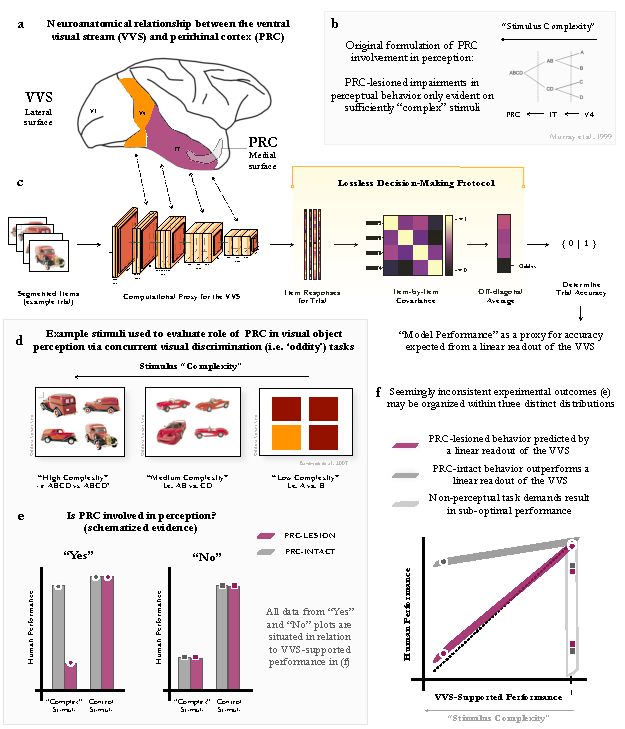
\includegraphics[width=.8\linewidth]{figures/F1}
\caption{\textbf{Resolving seemingly inconsistent experimental findings with a computational proxy for the ventral visual stream. (a)} Perirhinal cortex (PRC) is a neuroanatomical structure within the medial temporal lobe (MTL) situated at the apex of the ventral visual system (VVS), downstream of `high-level' visual structures such as inferior temporal (IT) cortex. \textbf{(b)} A perceptual-mnemonic hypothesis posits that PRC enables perceptual behaviors not supported by canonical sensory cortices, in addition to its mnemonic functions. Critically, PRC-related perceptual impairments are only expected on so-called ``complex'' perceptual stimuli. \textbf{(c)} Our trial-level protocol formalizes perceptual demands on PRC in concurrent visual discrimination (i.e. `oddity') tasks. We segment each stimulus screen containing N objects into N independent images, pass them to a computational proxy for the VVS, and extract N feature vectors from an `IT-like' layer. After generating a item-by-item covariance matrix for each trial, the item with the least off-diagonal covariance is marked as the `oddity.' Critically, this is a lossless decision-making protocol which is agnostic to extra-perceptual task demands (i.e. memory, attention, motivation). \textbf{(d)} Example stimuli used to evaluate the perceptual-mnemonic hypothesis that span the range of stimulus `complexity.' \textbf{(e)} Evaluating PRC involvement in perception has historically been formatted in categorical terms, and been forced to rely on with \emph{descriptive} accounts of stimulus properties (e.g. stimulus ``complexity''). This has generated seemingly inconsistent experimental evidence both for (left) and against (right) PRC involvement in perception. \textbf{(f)} Here we propose to resolve these apparent inconsistencies using this null model of PRC involvement in oddity tasks by identifying three distinct distributions in the literature: PRC-lesioned behavior that is predicted by a linear readout of the VVS, PRC-intact behavior that outperforms a linear readout of the VVS, and stimuli for which non-perceptual task demands result in sub-optimal performance. We consider experiments described as `complex' but which the model performs at ceiling (i.e. x=1) to be misclassified. }
\label{fig:PMA}
\end{figure}

% PRC-MODEL CORRESPONDENCE
\begin{figure}[ht]
\centering
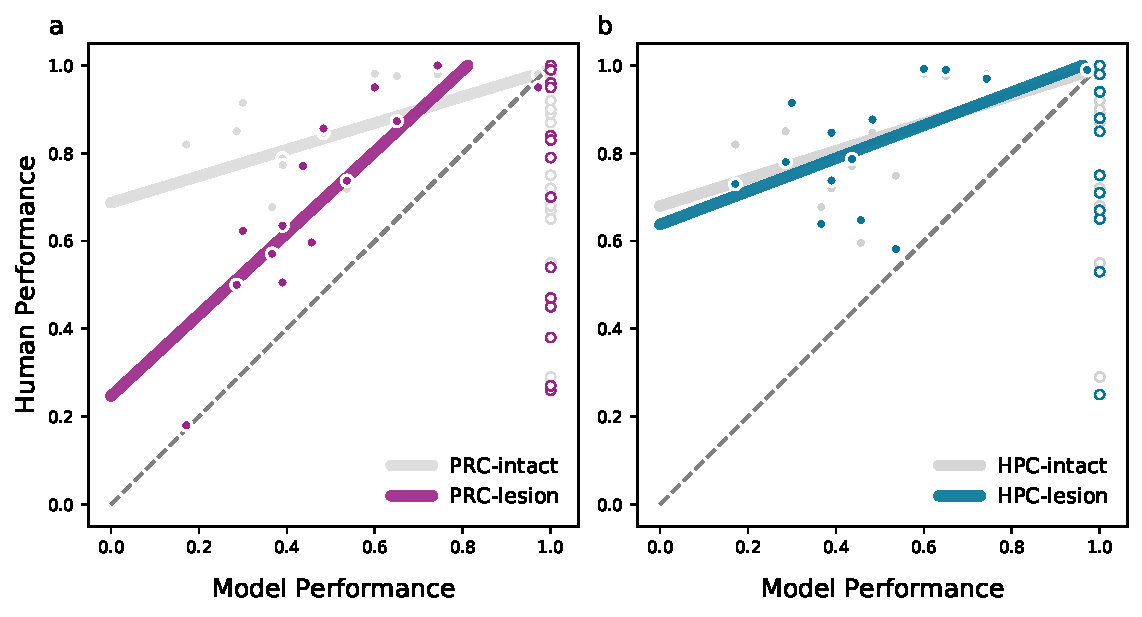
\includegraphics[width=\linewidth]{figures/F2}
\caption{\textbf{After excluding PRC-irrelevant stimuli, a computational proxy of the VVS predicts PRC-lesioned performance directly from experimental stimuli, while each are outperformed by PRC-intact participants.} We collect previously published `oddity' tasks administered to PRC-lesioned and -intact human participants. We then build a linear decoder off `IT-like' layers from a computational proxy for the VVS in order to determine the average performance across all trials in each experiment. This single value, model performance, corresponds to the experimental accuracy expected from a linear readout of IT cortex under a lossless decision-making protocol. Stimuli where model performance is at ceiling (x=1, open dots) are not relevant for evaluating the role of PRC in perception: As VVS responses should support perfect discrimination between these stimuli, any below ceiling performance in the human is attributed to extra-perceptual task demands (i.e. memory). \textbf{(a)} This computational proxy for IT cortex predicts the behavior of PRC-lesioned participants, while PRC-intact participants outperform both model and PRC-lesioned participants. \textbf{(b)} HPC-lesioned and intact participants all outperform this computational model on relevant stimuli; both for participants with an entirely intact medial temporal lobe, which includes PRC, as well as participants with selective damage to the hippocampus that spare PRC. Together, these results suggest that PRC-lesioned behavior reflects a linear readout of the VVS, neurotypical behaviors on these tasks outperform the VVS, and this behavior is dependent on PRC.}
\label{fig:prc_main}
\end{figure}

% VVS RELIANCE
\begin{figure}[ht]
\centering
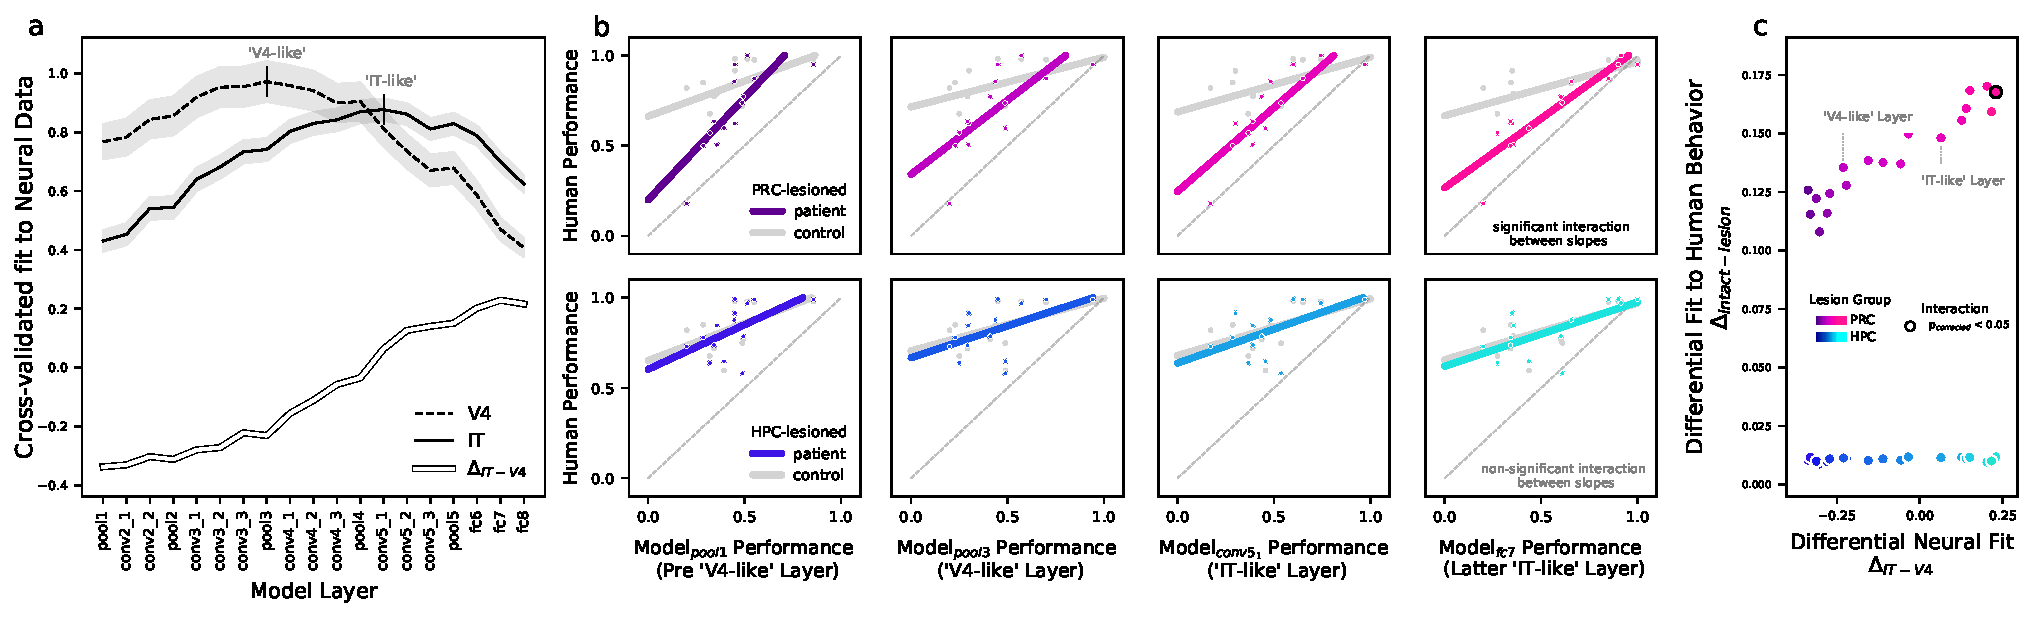
\includegraphics[width=\linewidth]{figures/F3}
\caption{\textbf{VVS reliance in a PRC-lesioned state: While `IT-like' model layers predict perirhinal-lesioned behaviors, the available stimuli do not clearly separate IT- from V4-supported performance.} There has long been concern that concurrent damage in PRC-adjacent cortical structures (such as IT) leads to perceptual deficits, not damage to PRC per se. These concerns are allayed by the observation that IT-like layers fail to perform `complex’ oddity tasks. Nonetheless, a question remains: where in the VVS is PRC-lesioned behavior reliant on? To address this question, we leverage the model's differential correspondence with V4 and IT electrophysiological responses across layers. \textbf{(a)} For each layer, we estimate the noise-corrected, cross-validated fit to electrophysiological responses in macaque IT and V4. We then compute each layer's differential fit to IT ($\Delta_{IT-V4}$: hollow). \textbf{(b)} Using the retrospective stimulus set, we determine each layer's differential fit to lesioned behavior, both for PRC- and HPC-lesioned participants (top and bottom panels, respectively), using the mean squared prediction error (MSPE) between human and model behavior. We then compute the difference between lesioned and intact model fits at each layer ($\Delta_{lesion}$ = MSPE$_{intact}$ - MSPE$_{lesion}$), for both PRC- and HPC-lesioned groups (e.g. $\Delta_{prc}$ = MSPE$_{prc.intact}$ - MSPE$_{prc.lesion}$). Additionally, we determine whether the interaction between lesioned and intact subject behavior is significant, repeating previous analyses (from Fig. \ref{fig:prc_main}a) across all layers. \textbf{(c)} Model layers that better fit IT cortex ($\Delta_{IT-V4}$) are better predictors of differential fit with PRC-reliant behavior ($\Delta_{prc}$, top). Additionally, the interaction between PRC-intact and -lesioned performance is only significant in `IT-like' layers, after correcting for multiple comparisons (black outlined circles). There is no correspondence between ($\Delta_{IT-V4}$) and HPC-lesioned behavior ($\Delta_{hpc}$, bottom). However, when directly comparing the model fit to PRC-lesioned participants in `IT-like' and `V4-like' model layers, there is not a significant difference, as can be seen in the relative similarity in the model fit to PRC-lesioned behaviors across all layers in (b). While these data suggest that PRC-lesioned behavior is reliant on high-level visual cortex, the available stimuli in the retrospective dataset do not enable focal anatomical claims.}
\label{fig:vvs_reliance}
\end{figure}

% NOVEL PROTOCOL
\begin{figure}[ht]
\centering
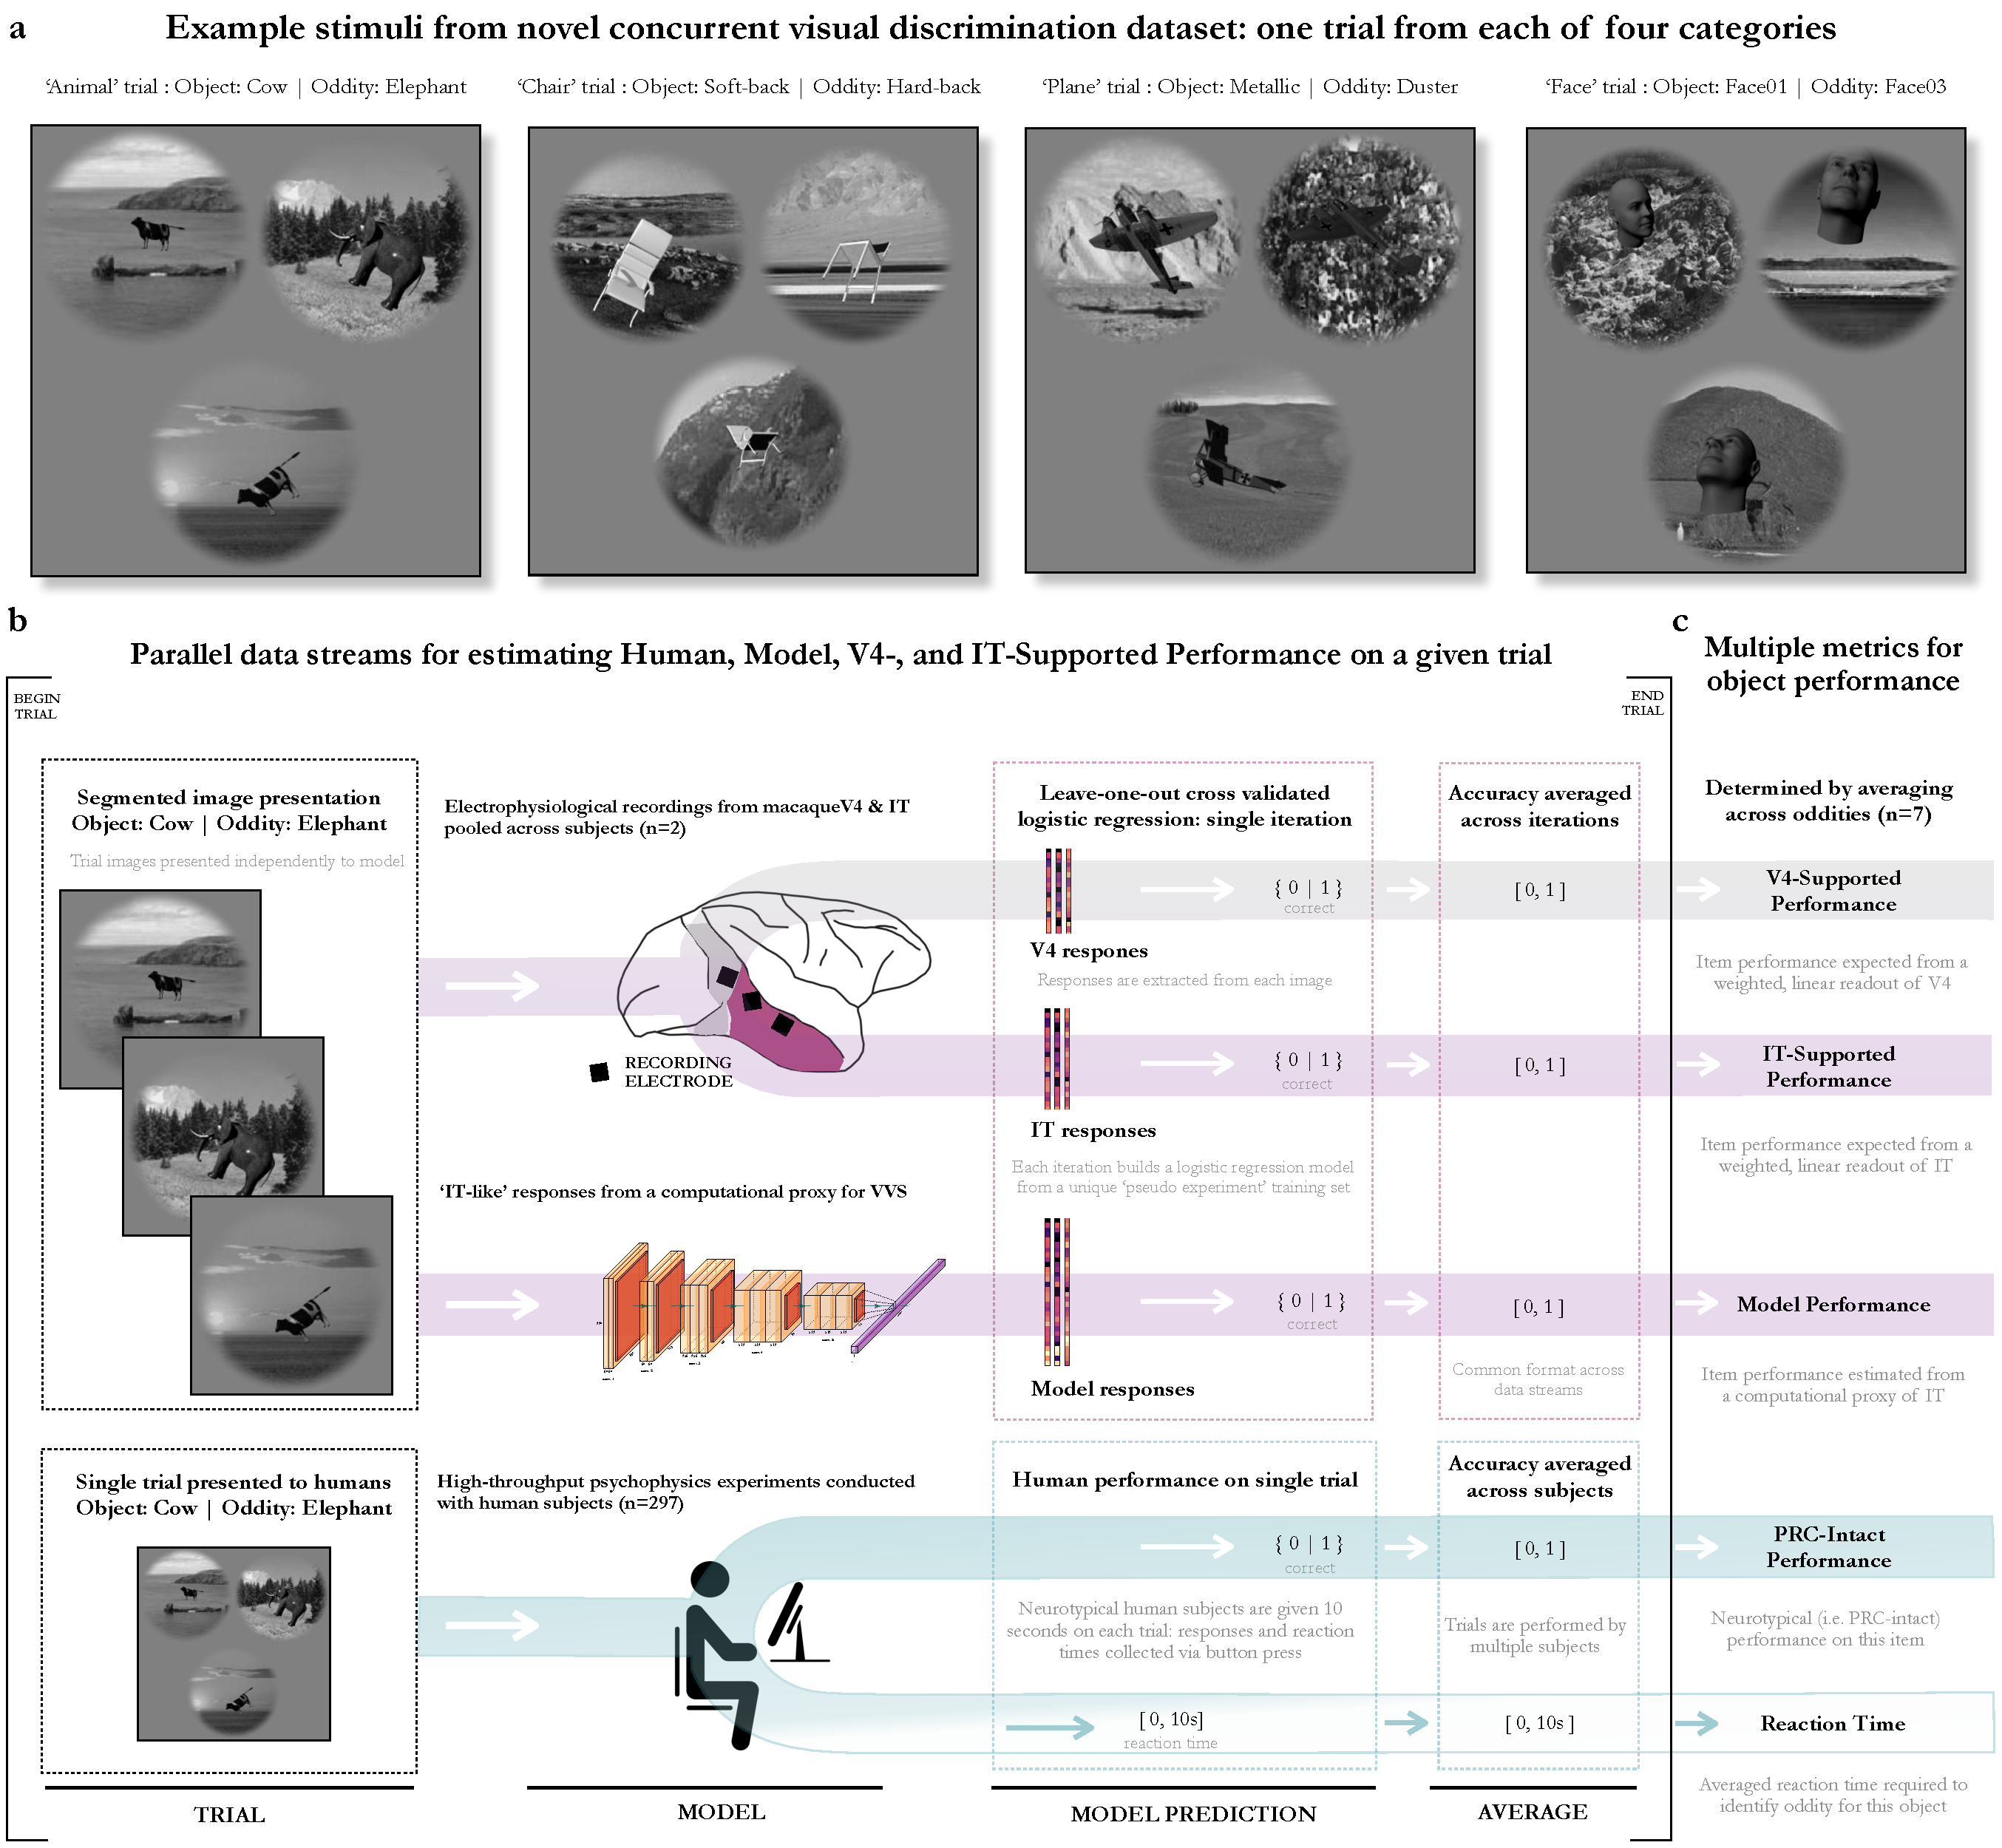
\includegraphics[width=\linewidth]{figures/F4}
\caption{\textbf{Parallel data processing streams enable comparison of VVS-supported performance, model performance, and PRC-Intact Performance on novel experimental stimuli} \textbf{(a)} Example stimuli from four categories used in the novel, model-driven concurrent visual discrimination experiment: together, this stimulus set contains 32 unique objects used to generate 224 unique within-category object combinations. \textbf{(b)} For each trial, given the same object and oddity images (left), there are parallel data processing streams to estimate human performance and Reaction time (RT), model performance, as well as V4- and IT-Supported Performance. Human data (bottom) are collected via high-throughput psychophysics experiments online: for a given trial, accuracy and RT data are collected, which are averaged across participants. To estimate model performance on these same stimuli (middle), objects are segmented and presented to the model, responses are extracted from an IT-like layer, a prediction is made using a modified leave-one-out cross-validated approach, and the average accuracy across iterations is taken as this trial's estimate of model performance. To estimate V4- and IT-Supported Behavior (top), we use the same protocol developed for the model, but predictions are made over electrophysiological recordings collected from the macaque\cite{majaj2015simple} instead of model responses. \textbf{(c)} To estimate performance on each unique object in this stimulus set (n=32), we take the average value collected across that object with all seven of its oddities. This yields human performance, model performance, as well as V4- and IT-Supported Performance on the same experimental stimuli. Colors matched to Fig. \ref{fig:novel_diagnostic}.}
\label{fig:novel_protocol_flow}
\end{figure}

% NOVEL DIAGNOSTIC STIMULI
\begin{figure}[ht]
\centering
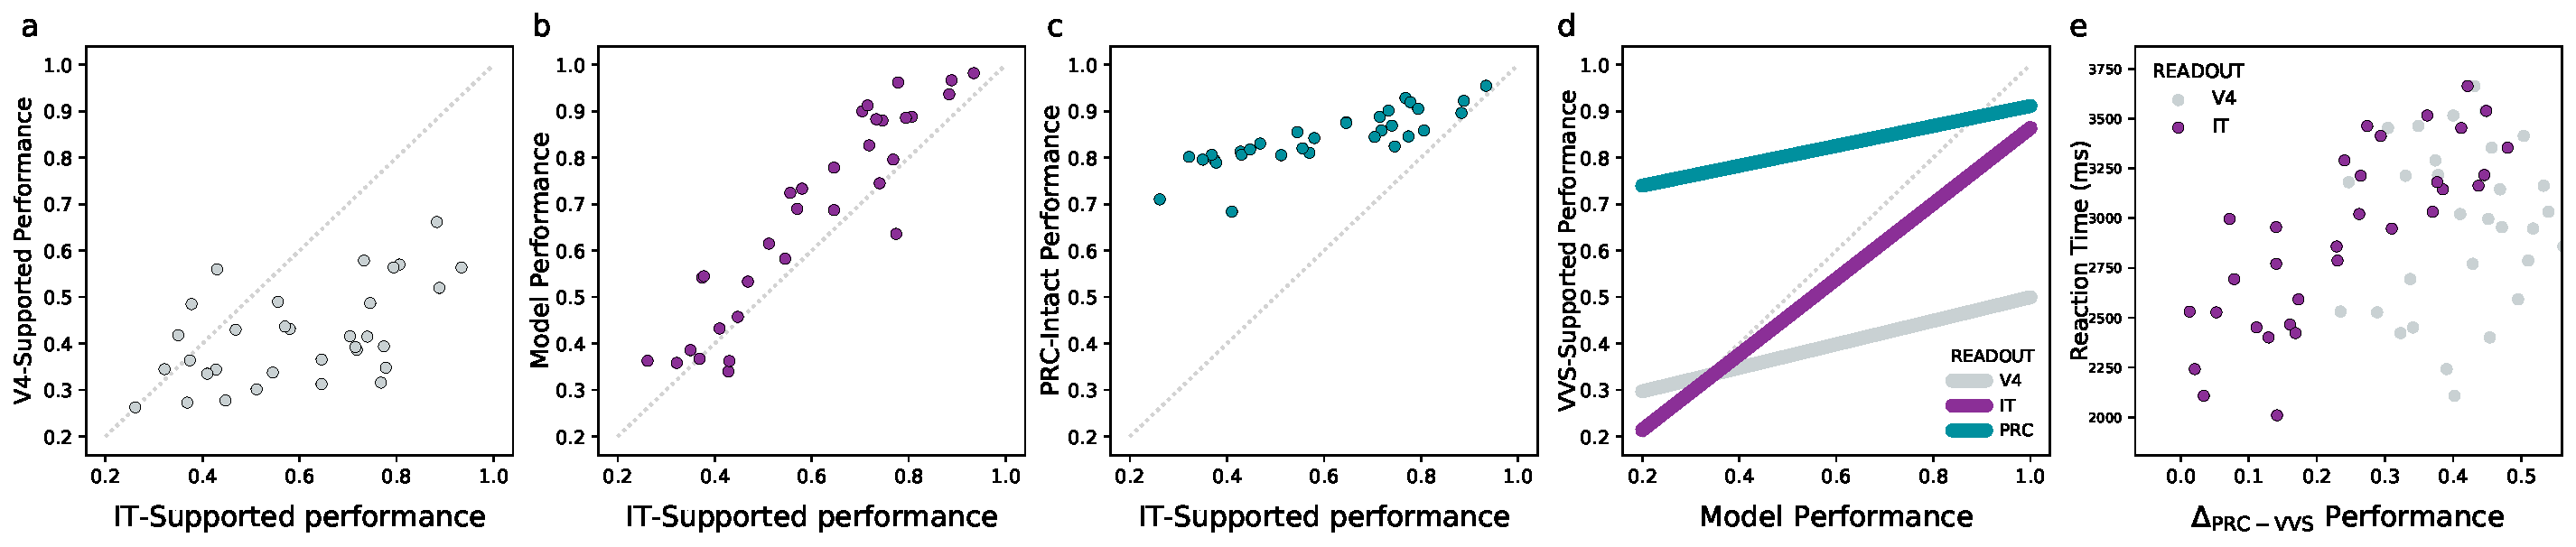
\includegraphics[width=\linewidth]{figures/F5}
\caption{\textbf{A model-driven stimulus set separates perirhinal-dependent behaviors from multiple stages of processing throughout the ventral visual system.} Here we evaluate the relationship between model, electrophysiological, and human performance on a novel stimulus set, generated within this modeling approach. \textbf{(a)} A weighted, linear readout of IT outperforms V4, clearly separating early from late stage processing within the VVS. \textbf{(b)} Model performance on these stimuli corresponds to IT-Supported Performance, validating the use of this model as a computational proxy for IT in oddity tasks. \textbf{(c)} Neurotypical (i.e. PRC-intact) human participants outperform V4- and IT-supported behavior, replicating findings from the retrospective analysis with a stimulus set that more densely and continuously samples the space of VVS-supported behavior. Additionally, these predictions are at the item level (averaged across oddities, $N=7$), not experimental averages. \textbf{(d)} The model provides a basis space to situate human behavior in relationship with VVS-supported performance, enabling more focal neuroanatomical claims about VVS-reliance in this and future experiments. \textbf{(e)} The difference between PRC-intact and IT-supported performance on each item scales with reaction time. These data suggest that in order to outperform a linear readout of IT cortex, PRC-intact participants require more time.}
\label{fig:novel_diagnostic}
\end{figure}

% RESNET ANALYSIS
\begin{figure}[ht]
\centering
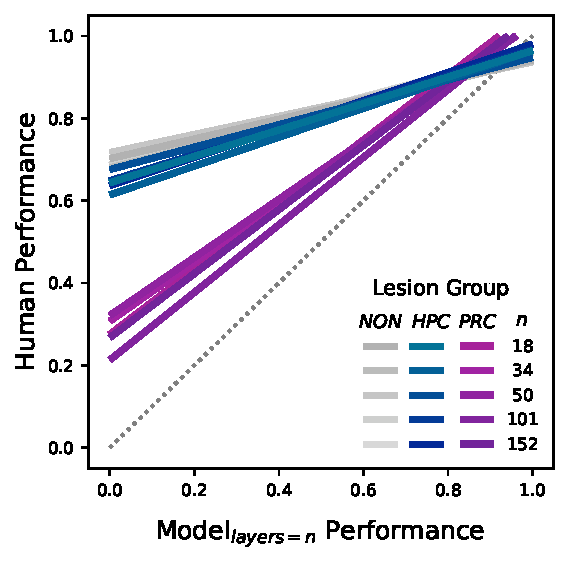
\includegraphics[width=.7\linewidth]{figures/F6}
\caption{\textbf{Increasing architecture depth does not achieve PRC-intact performance.} Here we repeat previous analyses but systematically vary model `depth' from 18-152 layers. For each of these architectures, we determine model performance for each experiment within the retrospective dataset. First we determine the model-selected oddity in each trial by identifying the item with the lowest off-diagonal correlation to the other items---as described in the retrospective analysis---using a penultimate, `IT-like' model layer; we then average the model's accuracy across all trials within an experiment. We compare model performance to PRC-intact (greys), HPC-lesioned (blues) and PRC-lesioned (purples) behavior for each model. Solid lines correspond to the best fit across all experiments. The interaction between PRC-intact and -lesioned subject behavior is persistent across all models. Increasing the number of VVS-like computations over a given stimulus–that is, by adding more layers–does not appear to approximate PRC-supported behaviors.}
\label{fig:layer_analysis}
\end{figure}

% TRAINING DATA FIGURE

%\begin{SCfigure}
%  \caption{This is the same picture of the universe as above, but now the captions appear in the side %next to the image}
%  \includegraphics[width=.5\textwidth]{universe}
%\end{SCfigure}

%\begin{SCfigure}
\begin{figure}[ht]
\centering
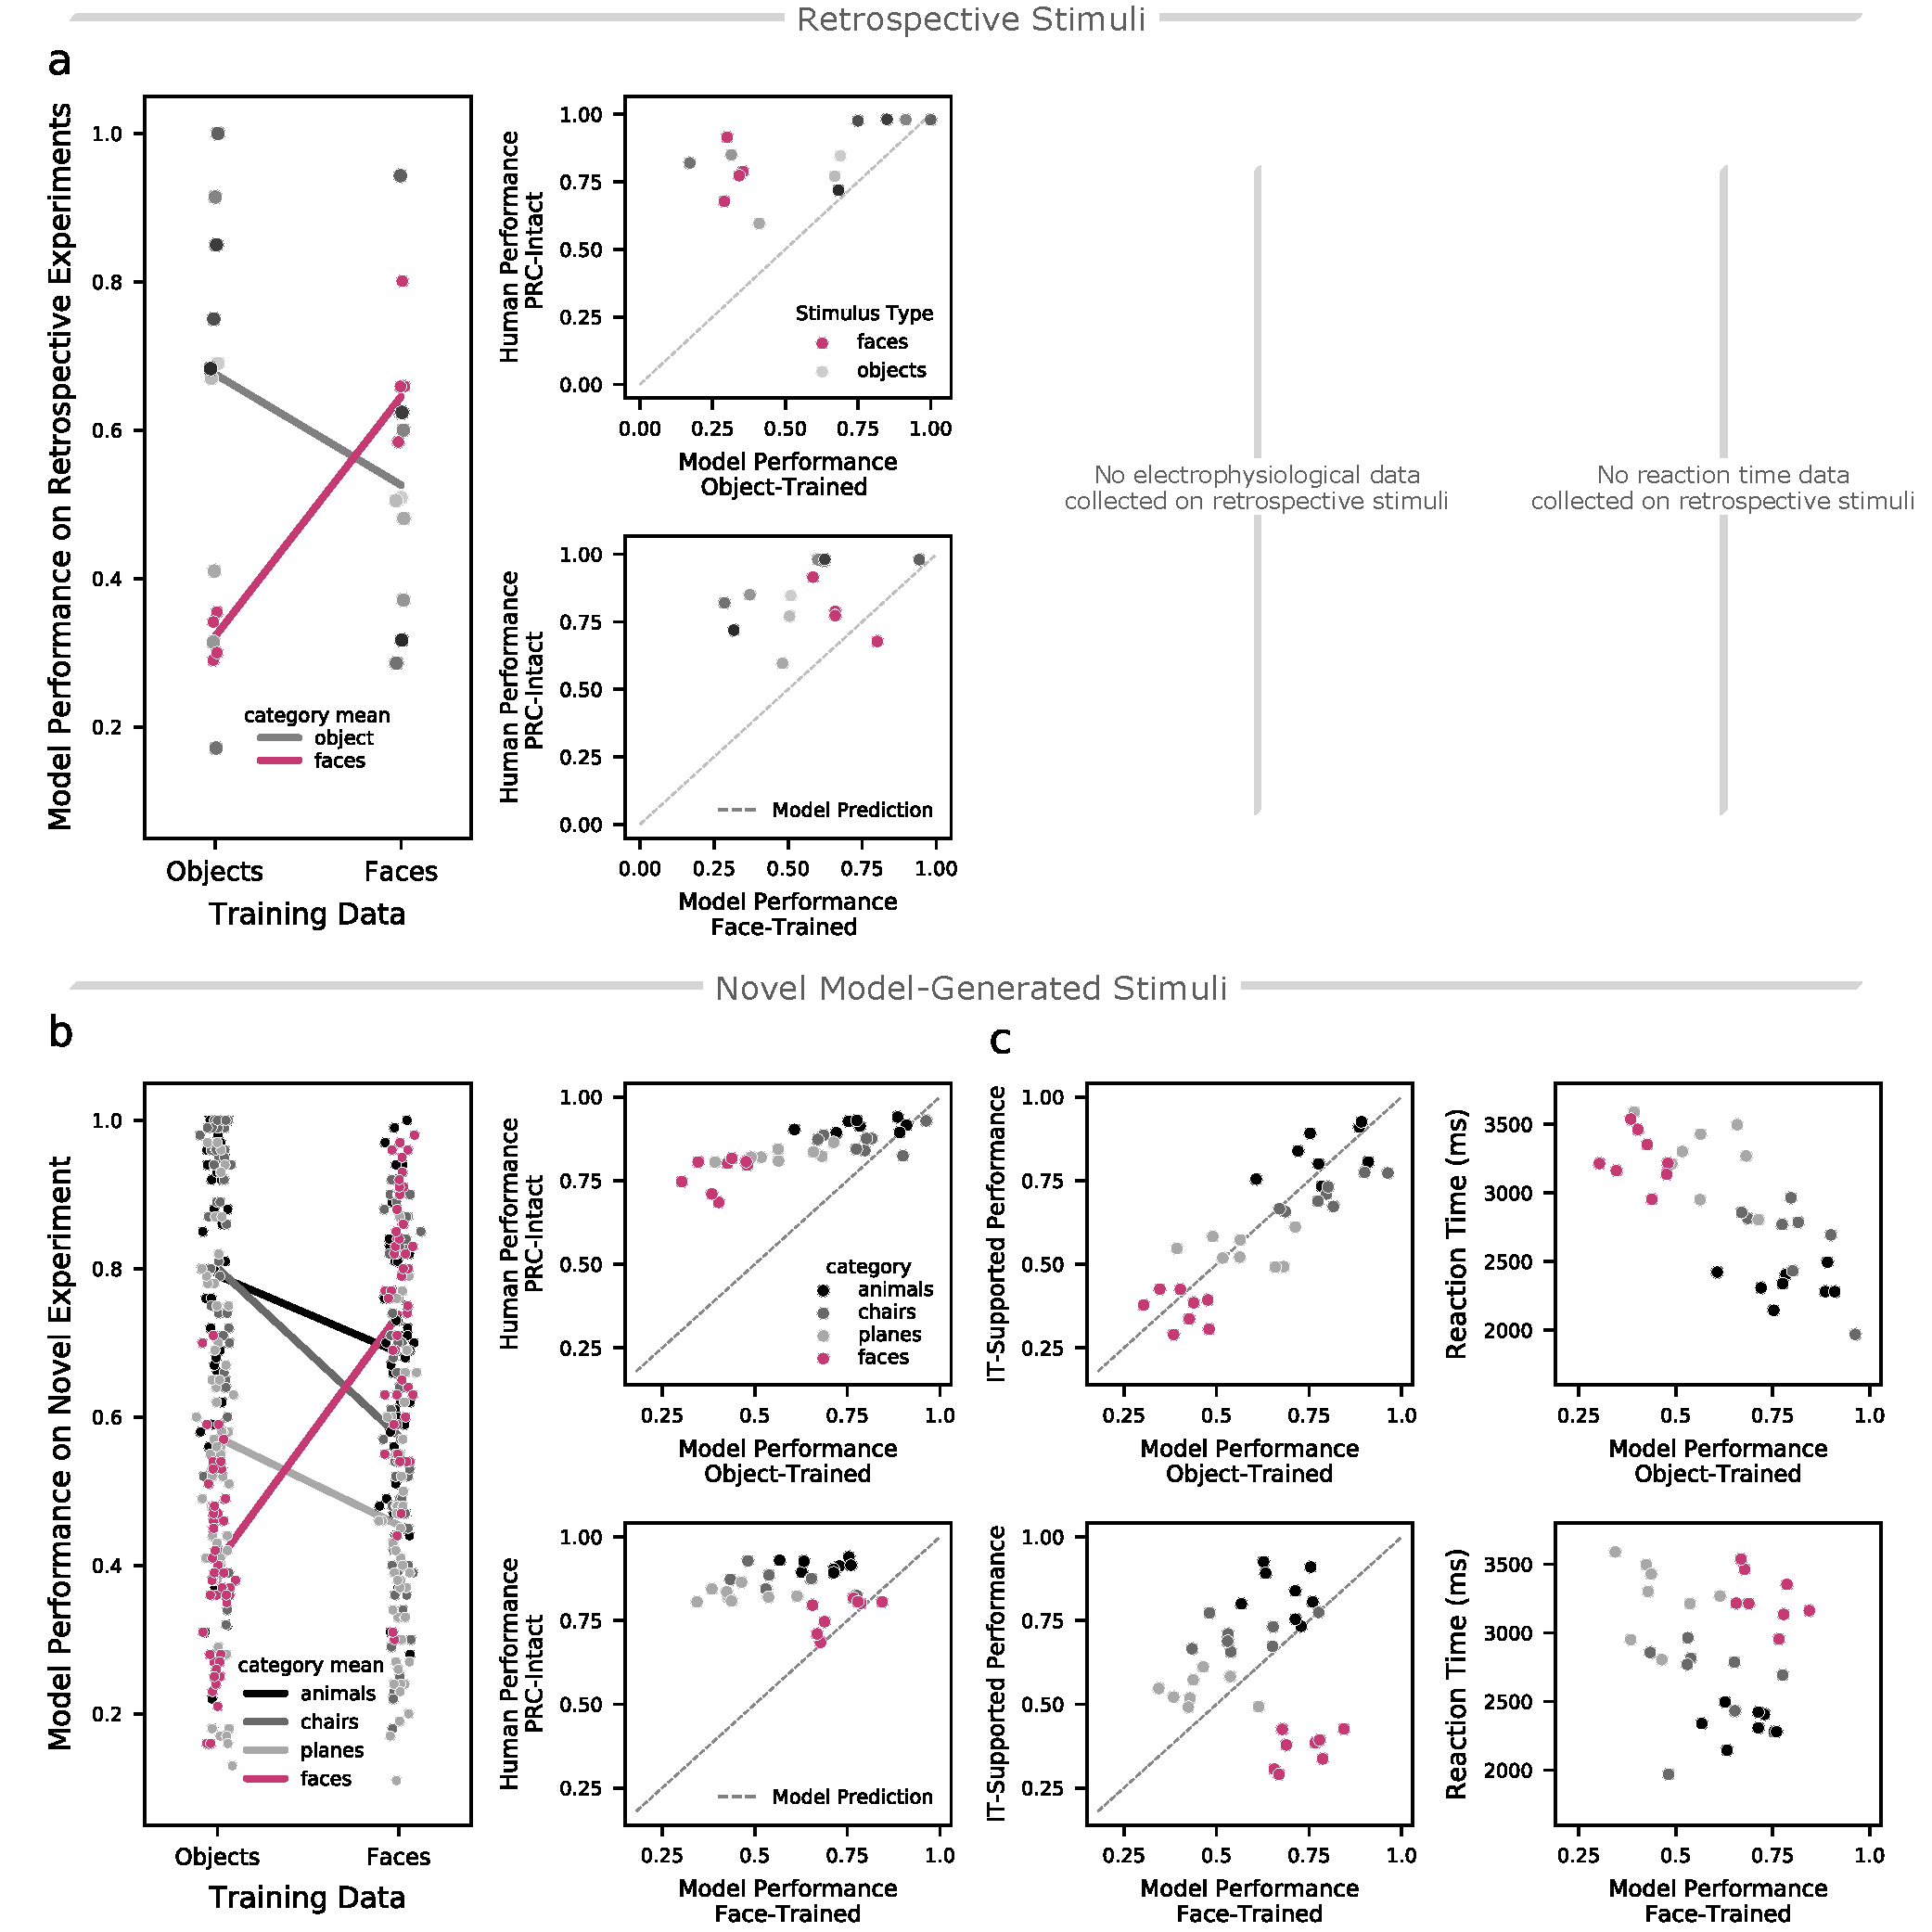
\includegraphics[width=.85\linewidth]{figures/F7}
\caption{\textbf{A computational proxy for the VVS achieves PRC-intact performance on `complex' stimuli, with training, but fails to generalize.} Faces are an example of putatively ‘complex’ experimental stimuli: VVS-like models, PRC-lesioned participants, and IT-supported performance all fail to approximate PRC-intact behaviors on this stimulus class. We optimize a computational proxy for the VVS to perform these ‘complex’ tasks by changing the distribution of its training data (i.e. using a dataset with millions of faces) and compare its behavior with a model optimized for a more domain general task of object categorization. \textbf{(a)} This content-specific optimization leads to increased model performance on `within distribution' stimuli in the retrospective dataset, while not generalizing to out-of-distribution stimuli; models optimized for face discrimination perform face-oddity tasks better than models optimized to perform object classification (red, left), while models optimized for objects classification better perform object-oddity tasks (grey, left). Comparing to human performance on faces in the retrospective dataset, object-trained models are significantly outperformed by PRC-intact participants (top right), while face-trained models exhibit performance that is not significantly different from PRC-intact behavior (bottom right). This pattern of results suggests that performance gains scale with the relative similarity of testing and training data, not stimulus properties, per se. \textbf{(b)} We replicate findings from the retrospective analysis using the novel, model-driven experimental stimuli: Models optimized for ‘complex’ visual content significantly outperform other models on ‘within distribution’ stimuli in the novel experiment (red, left), while exhibiting degraded performance on out-of-distribution stimuli (grey, left). Comparing to human performance on faces in the novel experiment, while object-trained models are significantly outperformed by PRC-intact participants (top right), face-trained models exhibit performance that is not significantly different from PRC-intact behavior (bottom right). \textbf{(c)} Model’s optimized for object classification recapitulate the performance supported by IT (top left) and reaction time of PRC-intact human subjects (top right). In contrast, this content-specific optimization breaks the correspondence between the model and IT-supported behavior (bottom left) and reaction time (botom right); while this optimization procedure leads to performance comparable to PRC-intact behavior on the trained stimulus type, these models should be considered to offer a solution to these tasks unlike PRC-dependent computations. Together, these results demonstrate that a content-specific optimization procedure enables VVS-like architectures to discriminate between `complex' stimuli, reflecting numerous findings from perceptual learning in the biological system. These computational results suggests that PRC-dependence on `complex' stimuli is not about stimulus properties, per se, but the interaction between stimulus properties and stimulus-relevant experience.
}
%\caption{\textbf{Synthetic `experiments': With training, a computational proxy for the VVS achieves PRC-intact performance on `complex' stimuli, but fails to generalize to stimuli unlike the training data.} Faces are an example of putatively ‘complex’ experimental stimuli: VVS-like models, PRC-lesioned participants, and IT-supported performance all fail to approximate PRC-intact behaviors on this stimulus class. We optimizing a computational proxy for the VVS to perform these ‘complex’ tasks by changing the distribution of its training data (i.e. using a dataset with millions of faces) and compare its behavior with model optimized for a more domain general task of object categorization. \textbf{(a)} This content-specific optimization leads to increased model performance on `within distribution' stimuli in the retrospective dataset, while not generalizing to out-of-distribution stimuli; models optimized for face discrimination perform face-oddity tasks better than models optimized to perform object classification (red, right), while models optimized for objects classification better perform object-oddity tasks (grey, left). Comparing to human performance on faces in the retrospective dataset, \textbf{(b)} object-trained models are significantly outperformed by PRC-intact participants, \textbf{(c)} while face-trained models exhibit performance that is not significantly different from PRC-intact behavior. This pattern of results suggests that performance gains scale with the relative similarity of testing and training data, not stimulus properties, per se. \textbf{(d)} We replicate findings from this analysis using the novel, model-driven experimental stimuli: Models optimized for ‘complex’ visual content significantly outperform other models on ‘within distribution’ stimuli in the novel experiment (red, right), while exhibiting degraded performance on out-of-distribution stimuli (grey, right). Comparing to human performance on faces in the novel experiment, \textbf{(e)} while object-trained models are significantly outperformed by PRC-intact participants, \textbf{(f)} face-trained models exhibit performance that is not significantly different from PRC-intact behavior. Additionally, \textbf{(g)} model’s optimized for object classification recapitulate the behavior supported by IT, \textbf{(h)} this content-specific optimization breaks the correspondence between model and IT-supported behavior. Similarly, while \textbf{(i)} models optimized to perform object classification predict the reaction time required to perform each trial, \textbf{(j)} this relationship is not present for this content-specific optimization procedure. The results suggest that while a content-specific optimization procedure (extensive training akin to perceptual learning) enables performance indistinguishable with PRC-intact participants, this approach does not reflect the underlying computations supported by PRC.}
\label{fig:traintest}
\end{figure}
%\end{SCfigure}

%%%%%%%%%%%%%%%%%%%%%%%%%%%%%%%%%%%%%%%%%%%%%%%%%%%%%%%%%%%%%%%%%%%%%%%%%%%%%%%%%%%%%%%%
\beginsupplement

% DIFFERENT READOUTS
\begin{figure}[ht]
\centering
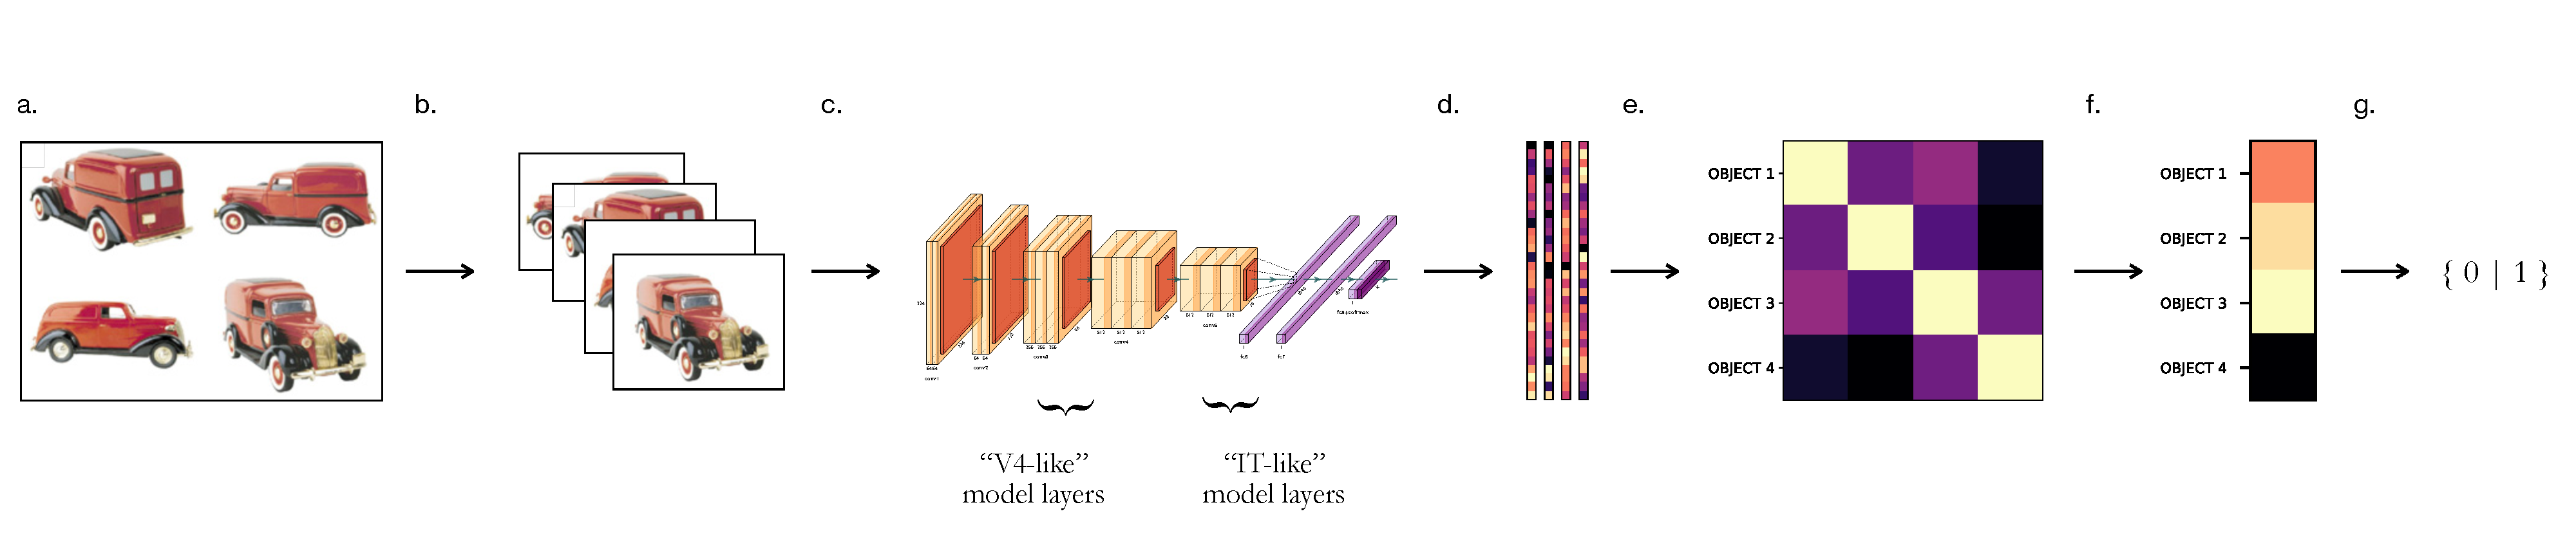
\includegraphics[width=\linewidth]{figures/S1}
\renewcommand{\figurename}{Supplementary Figure}
\caption{\textbf{ Experimental protocol for retrospective analyses}. \textbf{(a)} Each trial consists of a stimulus screen containing N objects. \textbf{(b)} These N objects are segmented into N object-centered images. \textbf{(c)} We pass these N object-centered images to the model, independently. \textbf{(d)} Using an “IT like” layer of the model, we extract model responses to the N objects, which are flattened into length F vectors, resulting in an FxN response matrix for each trail. \textbf{(e)} To identify the item-by-item similarity between objects, we use the Pearson’s correlation between items in this FxN response matrix, generating an NxN correlation matrix. \textbf{(f)} We average over each item's off-diagonal correlations, generating a single vector that corresponds to each items correlation with all other items. \textbf{(g)} We select the item with the lowest value as the model-selected oddity (e.g. bottom, the item least like the others). This model-selected oddity is labeled as either correct or incorrect, depending on its correspondence with ground truth.}
\label{fig:retrospective_protocol}
\end{figure}

% NON-DIAGNOSTIC STIMULI
\begin{figure}[ht]
\centering
\renewcommand{\figurename}{Supplementary Figure}
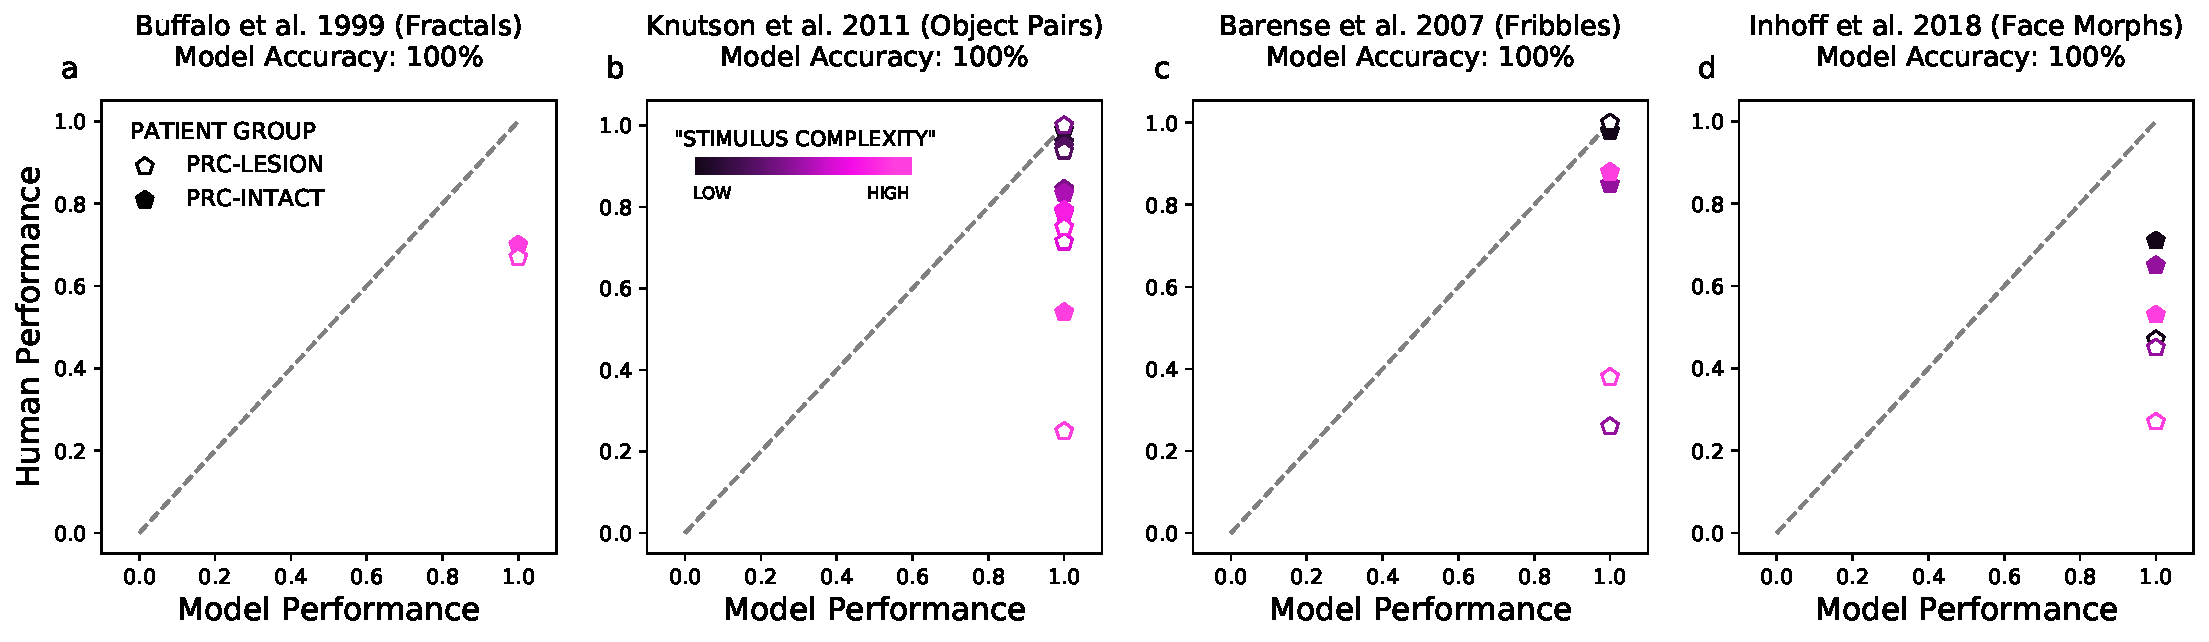
\includegraphics[width=\linewidth]{figures/S2}
\caption{\textbf{Stimulus sets appear to have been misclassified in the retrospective dataset, on both sides of the perceptual-mnemonic debate.} While the original authors described these experiments as `complex,' we find that they are perfectly computable by a computational proxy for the VVS (i.e. accuracy = 100\%). Below ceiling human performance on these experiments can be attributed to extra-perceptual task demands (e.g. memory), and so these experiments are not able to adjudicate PRC-involvement in perception. We separate these misclassified experiments into two categories. \textbf{(a-b)} There are eight experiments across two studies that were argued as evidence against perirhinal involvement in perception because performance did not significantly differ between PRC-intact and -lesioned participants. For these experiments, modeling results suggest that canonical VVS regions should be sufficient to meet the perceptual demands in these tasks, and thus the observed matched performance is expected. \textbf{(c-d)} There were six experiments that were argued to reveal evidence in support of perirhinal involvement in perception. While the authors argued that the observed deficits in PRC-lesioned participants are due to the perceptual demands imposed by these stimulus sets, the model revealed that they are perfectly computable by a computational proxy for the VVS, and so these deficits can be attributed to extra-perceptual task demands. Data in a-d are presented in Fig. \ref{fig:prc_main} at x=1.}
\label{fig:misclassified}
\end{figure}

% DIFFERENT READOUTS
\begin{figure}[ht]
\centering
%\renewcommand{\figurename}{Supplementary Figure}
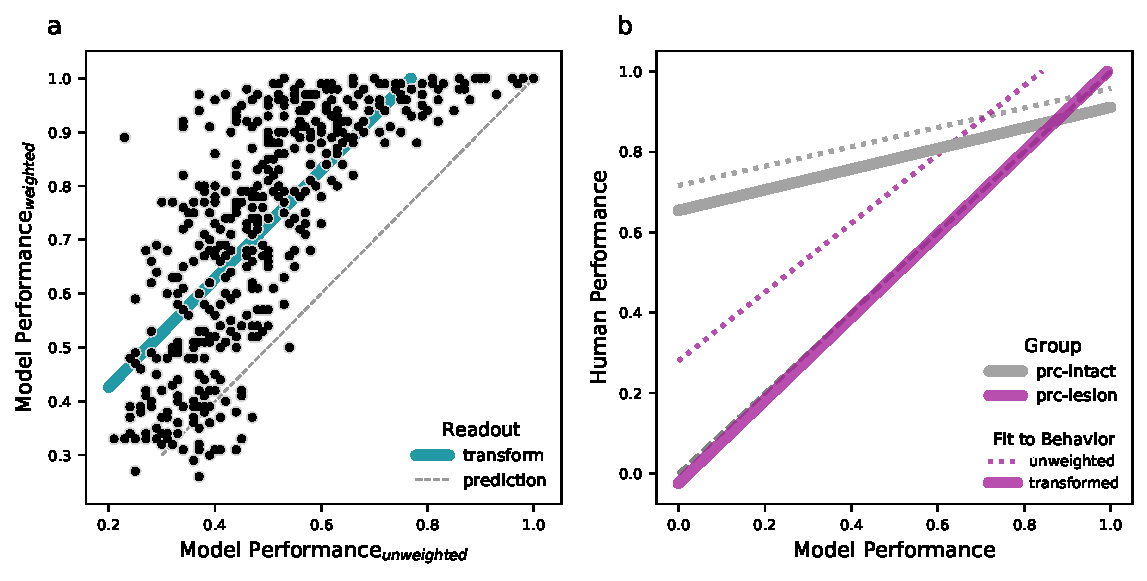
\includegraphics[width=\linewidth]{figures/S3}
\caption{\textbf{ Learning a weighted, linear readout of model features on trial-by-trial concurrent visual discrimination tasks improves the correspondence between model performance and PRC-lesioned behavior. (a)} A novel concurrent visual discrimination stimulus set densely and continuously spans the space of model performance defined using an unweighted linear (i.e. distance-based) readout of model responses (x axis), as per the original retrospective dataset analysis, and a weighted, linear readout of model responses learned through a leave-one-out cross-validation strategy (y axis). As expected, the learned, weighted readout outperforms the distance metric. We learn the transformation that projects the unweighted performance into the performance expected for the same stimuli using a learned, weighted readout (green). \textbf{(b)} Using the transform learned in (a), we project model performance supported by a uniform readout of model responses (i.e. the original retrospective analysis) into the performance that would be expected were it possible to learn a weighted readout on these stimuli. This improves the correspondence between model performance and human performance, motivating the need to use stimuli that enable a learned, weighted readouts of model performance.}
\label{fig:compare_readouts}
\end{figure}


% DIFFERENT READOUTS
\begin{figure}[ht]
\centering
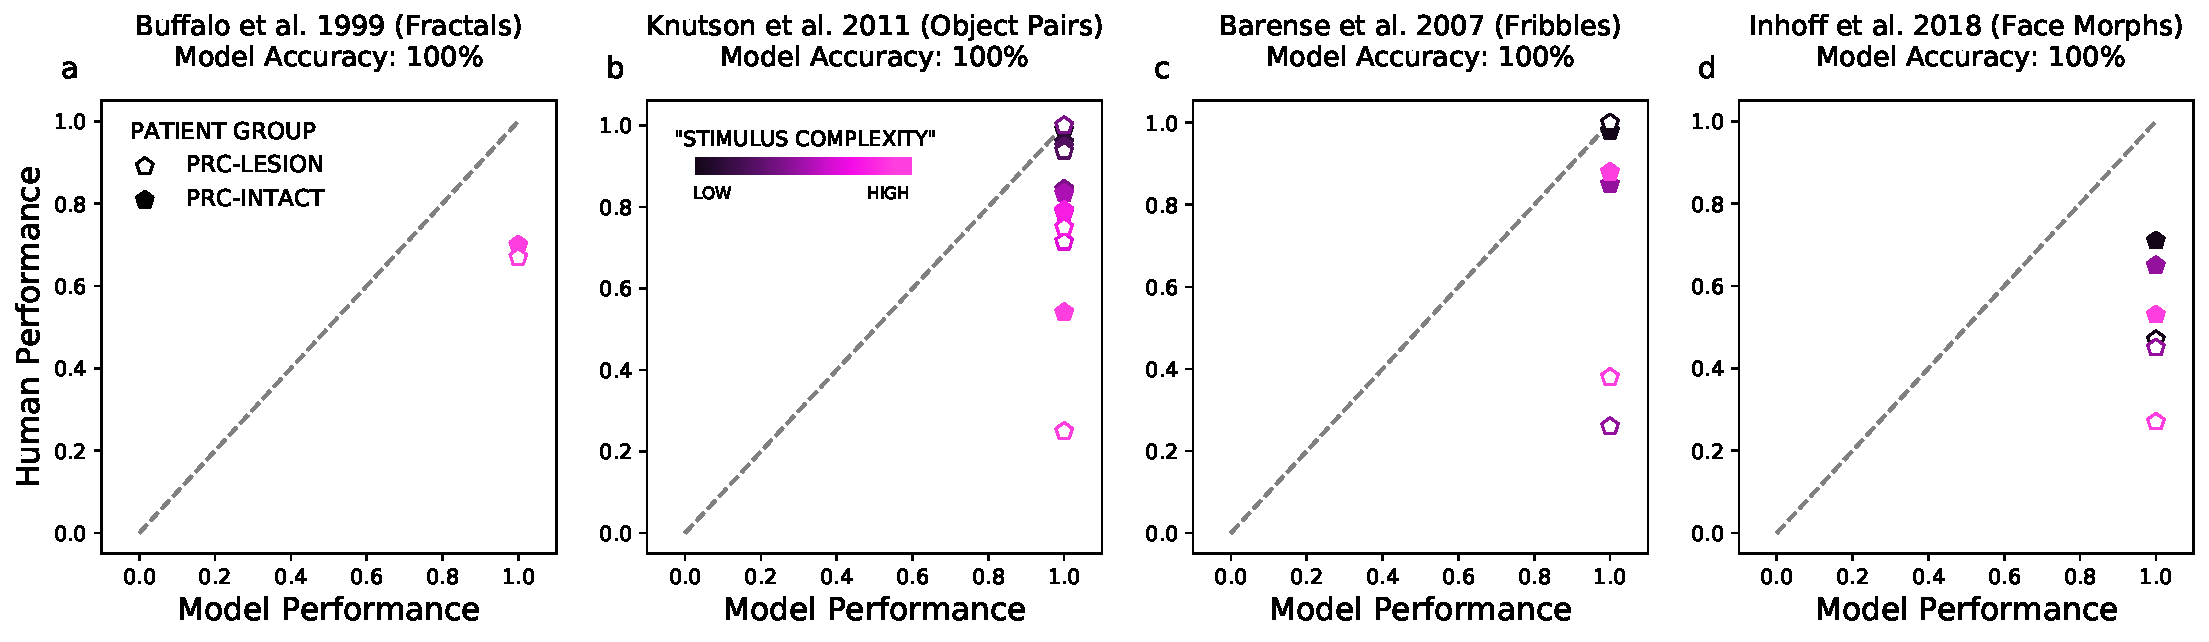
\includegraphics[width=\linewidth]{figures/S2}
\renewcommand{\figurename}{Supplementary Figure}
\caption{\textbf{ Without `foveating' stimuli before being presented to the model, content-specific optimization does not improves performance on `complex' experimental stimuli.} We optimize a computational proxy for the VVS to perform a ‘complex’ visual discrimination task---face identification---through perceptual training. In this approach, the images are presented to the model at central field of view, and encompass much of the available image. This is unlike the (previous) model trained through object classification, which receives images with objects whose locations and viewpoints are highly variable across images. The novel stimulus set, however, contains faces and other objects that are located at random locations across the stimulus screen---unlike the distribution of training data in the face-trained model. \textbf{(a)} Model performance$_{faces}$ is not better on face discrimination in the novel dataset than model performance$_{objects}$---and it is significantly worse on all other object types. \textbf{(b)} While model performance$_{objects}$ is outperformed by PRC-intact participants across many items (top left), it nonetheless provides a good fit to IT-supported behavior (top center), and predicts human subject reaction time on these tasks (top right). Conversely, model performance$_{faces}$ is outperformed by PRC-intact participants across all items (bottom left), outperformed by IT-supported behavior across many items (bottom center), and demonstrates no correspondence with human reaction time on these tasks (bottom right). This content-specific optimization procedure fails to generalize to images with higher variance in object location, regardless of their stimulus type. These results further corroborating the restricted (i.e. 'near transfer') performance enhancements observed with this approach. All data reported in the main results, and in Fig. \ref{fig:traintest}b-c are determine by `foveating' the images in the novel dataset before presenting them to the model, rendering them more similar to the images used during model optimization.}
\label{fig:compare_readouts_unfoveated}
\end{figure}

\end{document}